\documentclass{mimosis}

\usepackage{metalogo}

%%%%%%%%%%%%%%%%%%%%%%%%%%%%%%%%%%%%%%%%%%%%%%%%%%%%%%%%%%%%%%%%%%%%%%%%
% Some of my favourite personal adjustments
%%%%%%%%%%%%%%%%%%%%%%%%%%%%%%%%%%%%%%%%%%%%%%%%%%%%%%%%%%%%%%%%%%%%%%%%
%
% These are the adjustments that I consider necessary for typesetting
% a nice thesis. However, they are *not* included in the template, as
% I do not want to force you to use them.

% This ensures that I am able to typeset bold font in table while still aligning the numbers
% correctly.
\usepackage{etoolbox}

\usepackage[binary-units=true]{siunitx}
\DeclareSIUnit\px{px}

\sisetup{%
  detect-all           = true,
  detect-family        = true,
  detect-mode          = true,
  detect-shape         = true,
  detect-weight        = true,
  detect-inline-weight = math,
}

%%%%%%%%%%%%%%%%%%%%%%%%%%%%%%%%%%
% \usepackage{amsmath}
%%%%%%%%%%%%%%%%%%%%%%%%%%%%%%%%%%

%%%%%%%%%%%%%%%%%%%%%%%%%%%%%%%%%%%%%%%%%%%%%%%%%%%%%%%%%%%%%%%%%%%%%%%%
% Hyperlinks & bookmarks
%%%%%%%%%%%%%%%%%%%%%%%%%%%%%%%%%%%%%%%%%%%%%%%%%%%%%%%%%%%%%%%%%%%%%%%%

\usepackage[%
  colorlinks = true,
  citecolor  = RoyalBlue,
  linkcolor  = RoyalBlue,
  urlcolor   = RoyalBlue,
  ]{hyperref}

\usepackage{bookmark}

%%%%%%%%%%%%%%%%%%%%%%%%%%%%%%%%%%%%%%%%%%%%%%%%%%%%%%%%%%%%%%%%%%%%%%%%
% Bibliography
%%%%%%%%%%%%%%%%%%%%%%%%%%%%%%%%%%%%%%%%%%%%%%%%%%%%%%%%%%%%%%%%%%%%%%%%
%
% I like the bibliography to be extremely plain, showing only a numeric
% identifier and citing everything in simple brackets. The first names,
% if present, will be initialized. DOIs and URLs will be preserved.

\usepackage[%
  autocite     = plain,
  backend      = bibtex,
  doi          = true,
  url          = true,
  giveninits   = true,
  hyperref     = true,
  maxbibnames  = 99,
  maxcitenames = 99,
  sortcites    = true,
  style        = numeric,
  ]{biblatex}

%%%%%%%%%%%%%%%%%%%%%%%%%%%%%%%%%%%%%%%%%%%%%%%%%%%%%%%%%%%%%%%%%%%%%%%%
% Some adjustments to make the bibliography more clean
%%%%%%%%%%%%%%%%%%%%%%%%%%%%%%%%%%%%%%%%%%%%%%%%%%%%%%%%%%%%%%%%%%%%%%%%
%
% The subsequent commands do the following:
%  - Removing the month field from the bibliography
%  - Fixing the Oxford commma
%  - Suppress the "in" for journal articles
%  - Remove the parentheses of the year in an article
%  - Delimit volume and issue of an article by a colon ":" instead of
%    a dot ""
%  - Use commas to separate the location of publishers from their name
%  - Remove the abbreviation for technical reports
%  - Display the label of bibliographic entries without brackets in the
%    bibliography
%  - Ensure that DOIs are followed by a non-breakable space
%  - Use hair spaces between initials of authors
%  - Make the font size of citations smaller
%  - Fixing ordinal numbers (1st, 2nd, 3rd, and so) on by using
%    superscripts

% Remove the month field from the bibliography. It does not serve a good
% purpose, I guess. And often, it cannot be used because the journals
% have some crazy issue policies.
\AtEveryBibitem{\clearfield{month}}
\AtEveryCitekey{\clearfield{month}}

% Fixing the Oxford comma. Not sure whether this is the proper solution.
% More information is available under [1] and [2].
%
% [1] http://tex.stackexchange.com/questions/97712/biblatex-apa-style-is-missing-a-comma-in-the-references-why
% [2] http://tex.stackexchange.com/questions/44048/use-et-al-in-biblatex-custom-style
%
\AtBeginBibliography{%
  \renewcommand*{\finalnamedelim}{%
    \ifthenelse{\value{listcount} > 2}{%
      \addcomma
      \addspace
      \bibstring{and}%
    }{%
      \addspace
      \bibstring{and}%
    }
  }
}

% Suppress "in" for journal articles. This is unnecessary in my opinion
% because the journal title is typeset in italics anyway.
\renewbibmacro{in:}{%
  \ifentrytype{article}
  {%
  }%
  % else
  {%
    \printtext{\bibstring{in}\intitlepunct}%
  }%
}

% Remove the parentheses for the year in an article. This removes a lot
% of undesired parentheses in the bibliography, thereby improving the
% readability. Moreover, it makes the look of the bibliography more
% consistent.
\renewbibmacro*{issue+date}{%
  \setunit{\addcomma\space}
    \iffieldundef{issue}
      {\usebibmacro{date}}
      {\printfield{issue}%
       \setunit*{\addspace}%
       \usebibmacro{date}}%
  \newunit}

% Delimit the volume and the number of an article by a colon instead of
% by a dot, which I consider to be more readable.
\renewbibmacro*{volume+number+eid}{%
  \printfield{volume}%
  \setunit*{\addcolon}%
  \printfield{number}%
  \setunit{\addcomma\space}%
  \printfield{eid}%
}

% Do not use a colon for the publisher location. Instead, connect
% publisher, location, and date via commas.
\renewbibmacro*{publisher+location+date}{%
  \printlist{publisher}%
  \setunit*{\addcomma\space}%
  \printlist{location}%
  \setunit*{\addcomma\space}%
  \usebibmacro{date}%
  \newunit%
}

% Ditto for other entry types.
\renewbibmacro*{organization+location+date}{%
  \printlist{location}%
  \setunit*{\addcomma\space}%
  \printlist{organization}%
  \setunit*{\addcomma\space}%
  \usebibmacro{date}%
  \newunit%
}

% Do not abbreviate "technical report".
\DefineBibliographyStrings{english}{%
  techreport = {technical report},
}

% Display the label of a bibliographic entry in bare style, without any
% brackets. I like this more than the default.
%
% Note that this is *really* the proper and official way of doing this.
\DeclareFieldFormat{labelnumberwidth}{#1\adddot}

% Ensure that DOIs are followed by a non-breakable space.
\DeclareFieldFormat{doi}{%
  \mkbibacro{DOI}\addcolon\addnbspace
    \ifhyperref
      {\href{http://dx.doi.org/#1}{\nolinkurl{#1}}}
      %
      {\nolinkurl{#1}}
}

% Use proper hair spaces between initials as suggested by Bringhurst and
% others.
\renewcommand*\bibinitdelim {\addnbthinspace}
\renewcommand*\bibnamedelima{\addnbthinspace}
\renewcommand*\bibnamedelimb{\addnbthinspace}
\renewcommand*\bibnamedelimi{\addnbthinspace}

% Make the font size of citations smaller. Depending on your selected
% font, you might not need this.
\renewcommand*{\citesetup}{%
  \biburlsetup
  \small
}

\DeclareLanguageMapping{british}{bibliography-correct-ordinals}
\DeclareLanguageMapping{english}{bibliography-correct-ordinals}

\bibliography{Thesis}

%%%%%%%%%%%%%%%%%%%%%%%%%%%%%%%%%%%%%%%%%%%%%%%%%%%%%%%%%%%%%%%%%%%%%%%%
% Fonts
%%%%%%%%%%%%%%%%%%%%%%%%%%%%%%%%%%%%%%%%%%%%%%%%%%%%%%%%%%%%%%%%%%%%%%%%

\ifxetexorluatex
  \setmainfont{Minion Pro}
\else
  \usepackage[lf]{ebgaramond}
  \usepackage[oldstyle,scale=0.7]{sourcecodepro}
  \singlespacing
\fi

\renewcommand{\th}{\textsuperscript{\textup{th}}\xspace}

\newacronym[description={Principal component analysis}]{PCA}{PCA}{principal component analysis}
\newacronym                                            {SNF}{SNF}{Smith normal form}
\newacronym[description={Topological data analysis}]   {TDA}{TDA}{topological data analysis}

\newglossaryentry{LaTeX}{%
  name        = {\LaTeX},
  description = {A document preparation system},
  sort        = {LaTeX},
}

\newglossaryentry{Real numbers}{%
  name        = {$\real$},
  description = {The set of real numbers},
  sort        = {Real numbers},
}

\makeindex
\makeglossaries

%%%%%%%%%%%%%%%%%%%%%%%%%%%%%%%%%%%%%%%%%%%%%%%%%%%%%%%%%%%%%%%%%%%%%%%%
% Incipit
%%%%%%%%%%%%%%%%%%%%%%%%%%%%%%%%%%%%%%%%%%%%%%%%%%%%%%%%%%%%%%%%%%%%%%%%

\title{\texttt{Polarization Enhanced Texture Analysis}}
\subtitle{With Applications to Precision Agriculture}
\author{Nicholas Ericksen}

\begin{document}

\frontmatter
  \begin{titlepage}
  \vspace*{5cm}
  \makeatletter
  \begin{center}
    \begin{Huge}
      \@title
    \end{Huge}\\[0.1cm]
    %
    \begin{Large}
      \@subtitle
    \end{Large}\\
    %
    \emph{by}\\
    \@author
    %
    \vfill
    A document submitted in partial fulfillment
    of the requirements for the degree of\\
    \emph{Master of Science}\\
    at\\
    \textsc{Manhattan College}
  \end{center}
  \makeatother
\end{titlepage}

\newpage
\null
\thispagestyle{empty}
\newpage

  \begin{center}
  \textsc{Abstract}
\end{center}
%
\noindent
%
As agricultural inputs, such as water and fertilizer, become more scarce in the future, a higher level of precision will be required when utilizing these resources. Remote sensing is a field that has aimed to understand data from radiation reflected from vegetation.  Remote determination of water content
of this vegetation remains a long term goal.  Furthermore as agricultural production has also shifted to indoor
growing environments, the use of indoor sensors at smaller scales could be useful for determining the
physiological status of crops. In this study the use of texture, polarization and pseudo-spectral features captured in
acquired images are shown to be useful for the successful classification of
three different deciduous tree species common to the northeastern part of the
United States using a linear support vector classifier. The observations
are extended to the intra-class variance of the derived features and are shown
to be useful for the prediction of the relative water content of individual leaves when
analyzed using support vector regression.

  \begin{center}
  \textsc{Acknowledgments}
\end{center}
%
\noindent
%
For my parents, family and friends who have continuously demonstrated support in my pursuit of happiness.


A special thanks to Dr. Romeo Pascone, Dr. George Giakos, and Dr. Mark DeBonis whose input on this journey has been of great benefit.


The work performed in obtaining the resulting data could not have been accomplished without support from the labs at Manhattan College in the areas of Exploratory Image Research, Biology and Environmental Engineering.


  \tableofcontents

\mainmatter

  %%%%%%%%%%%%%%%%%%%%%%%%%%%%%%%%%%%%%%%%%%%%%%%%%%%%%%%%%%%%%%%%%%%%%%%%
\chapter{Introduction}
%%%%%%%%%%%%%%%%%%%%%%%%%%%%%%%%%%%%%%%%%%%%%%%%%%%%%%%%%%%%%%%%%%%%%%%%

\begin{center}
  \begin{minipage}{0.75\textwidth}
    \begin{small}
      “The motion of a pendulum has exerted a fascination for human minds since the first savage watched the swaying of the first tree branch. The smooth sinusoidal motion back and forth, seems to express some secret of the universe…
      Indeed, nature loves the sinusoid”.\\
      \null\hfill\emph{Linear Circuits, Scott}
    \end{small}
  \end{minipage}
  \vspace{0.5cm}
\end{center}

\noindent The natural environment\cite{knuthwebsite} contains a finite amount of resources.  It provides a limiting principle to the uncontrolled, exponential capital growth of consumerism.  If ancient civilization describes itself as a political social animal, modern culture must append the term consumer. Consumption of these resources is occurring at an increasing rate, as the world’s population increases, putting a strain on the modern agricultural system.  In 1798 Thomas Malthus wrote in his “Essay on the Principal of Population” that the standard of living would eventually be undermined as population grows exponentially, and food supplies grow geometrically.  He predicted this would eventually lead to mass food shortages and famine.

Today precision agriculture attempts to reduce the number of inputs to a farm, while maximizing its outputs.  Its goal is the management of agricultural inputs on an individual plant basis.  Minimizing water and fertilizer inputs are of central importance to this problem.

The areas of remote sensing, image processing, and machine learning have all been aided by advances in modern computing power.  The application of these disciplines to areas of precision agriculture are widespread.

Remote sensing in particular has had a tremendous impact on precision agricultural as it opens up the possibility of large area surveying and field health assessment.  Recently satellite data has been made easily available to the public through hosting on Amazon Web Services S3 buckets.  They include data from Landsat 8, the Geostationary Operational Environmental Satellites (GOES), NASA Earth Exchange (NEX), and the National Agricultural Imagery Program (NAIP).  These datasets contain information on various spectral responses recorded by various satellites.  Some of the datasets also contain scenes captured through polarization filters oriented at various angles. These polarization images can be useful for deriving certain backscatter and volume scattering properties of the scene under investigation and have been utilized by [18, 21].

[CHECK] When interpreting data from remotely sensed imagery of vegetation, it is important to understand the scattering mechanisms inherent to the various features found within a particular image.  This includes scattering from background objects such as soil, man made objects, canopies, etc. as well as target objects such as crops. Canopies are made up of individual leaves.  It is important to understand the scattering mechanisms that occur from each leaf in order to gain an increased insight into the larger effects evident in canopies. More precise models can then be created for the purpose of extrapolating micro level effects to the macro level.

[CHECK] Furthermore, as more agricultural operations are moved indoors, information acquired from cameras monitoring these greenhouses can provide insights into the health and growth stages of various crops. Research into building greenhouses in space for the colonization of other planets, has always grown substantially as of late, with programs such as SpaceX looking into the possibility of placing a greenhouse on Mars.  This provides an opportunity for placing image sensors into confined growing areas for monitoring plants on a micro scale.

Vegetation indices (VI) have been created for quantifying the health of land plants from remotely sensed data.  These indices rely on the spectral signatures exhibited by plants that vary with the state of a vegetation’s health [12].  It is possible that these ideas can be applied to smaller scale indoor scenarios as well.

Additional image processing can result in texture features being extracted from images for the purposes of segmentation and texture based classification.  It has been found that certain materials when captured from satellites and other airborne imaging devices, exhibit texture signatures that can be useful for these purposes [19].

Machine learning techniques have been applied to a large number of different research areas.  Their usefulness for classification and regression problems in the agricultural and environmental fields has been demonstrated for the purposes of plant disease detection and prevention, plant discrimination, levee management, etc. [18, 20, 27, 28, 29].

As consumer drones have entered the marketplace, it has become more reasonable for smaller scale farmers to utilize these remote sensors for monitoring there fields.  Consumer off the shelf (COTS) cameras have also decreased in price, allowing for cheap installation and modification for the purpose of agricultural monitoring at different scales.

[CHECK] This work investigates the effects of light reflected from individual plant leaves by multiple scattering mechanisms using a COTS camera at a micro scale.  This information can be used for the purpose of classification and ultimately determining the health of a plant based on the physiological properties of individual leaves by observing their polarization and texture properties as detected by the camera.  As resources become more scare, and the price of certain technologies decreases, the impact of utilizing information acquired by these sensors for precision agricultural will be large.

  %%%%%%%%%%%%%%%%%%%%%%%%%%%%%%%%%%%%%%%%%%%%
\chapter{Background}
%%%%%%%%%%%%%%%%%%%%%%%%%%%%%%%%%%%%%%%%%%%%
\begin{center}
  \begin{minipage}{0.75\textwidth}
    \begin{small}
      “The interaction between material bodies can be described either by formuating the action at a distance between the interacting bodies or by separating the interaction process into the production of a field by one system and the action of the field on another system” .
      \emph{Classical Electricity \& Magnetism. Panofksy, Phillips}\\.
    \end{small}
  \end{minipage}
  \vspace{0.5cm}
\end{center}

%%%%%%%%%%%%%%%%%%%%%%%%%%%%%%%%%%%%%%%%%%%
\section{The Nature of Light and the Electromagnetic Spectrum}
%%%%%%%%%%%%%%%%%%%%%%%%%%%%%%%%%%%%%%%%%%%
Light is fundamental to life.  In Maxwell’s’ theory on light he explained how electromagnetic phenomenon can be expressed in terms of waves \cite{maxwell}.  These waves move at the speed of light.  The light that human eyes can detect is a small portion of the electromagnetic spectrum called ‘visible light’.
%
%CHECK [insert EM image here]
\begin{figure}[!htb]
    \begin{center}
        \makebox[\textwidth]{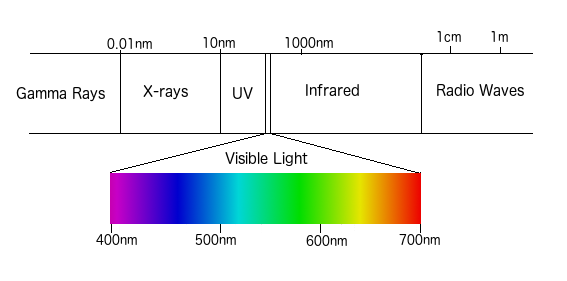
\includegraphics[scale=0.75]{/Sources/Background/Nature_of_Light/EM-spectrum.png}}
    \end{center}
    \caption{Electromagnetic Spectrum - Partial}
    \label{fig:polarization}
\end{figure}
Different frequencies of light correspond to different colors on the visible spectrum.  These waves are made up of two parts, the electric and magnetic.  Due to their similar nature often only the electrical portion is considered at first for mathematical simplicity.

The electrical portion of EM waves, and the only portion considered here, can be described as the sum of two sinusoidal waves representing the orthogonal x and y components in Cartesian space.
%
\begin{align}
    E(z,t)=E_x (t)+E_y (t)\\
    E_x (t)=E_{0x} cos( \theta+\delta_x )\\
    E_y (t)=E_{0y} cos( \theta+\delta_y )
\end{align}
%
where $ \theta = \delta t-kz $ is the wave propagator that determines the frequency and direction of propagation for the wave.$ \delta_y and \delta_x $ represent the phase delay for each component of the wave.

When more than one sine wave is considered, as in the case of EM waves, an overall phase delay between the them is considered and represented as $ \tau=\delta_y-\delta_x $.

Light can also be viewed as packets of energy known as photons.  The energy of photons is related to its frequency $v$ and a constant, known as Planck’s constant $h$ \cite{ecophysiology}.
%
\begin{align}
	h=6.62e-34 [m^2 kg/s]\\
	E=hv [Joules]
\end{align}
%
This simple equation shows that for higher frequencies, particles have higher energy.

%%%%%%%%%%%%%%%%%%%%%%%%%%%%%%%%%%%%%%%%%%%%%%%%%%%%%%%%%%%%%%
% Nature of Light Subsections
%%%%%%%%%%%%%%%%%%%%%%%%%%%%%%%%%%%%%%%%%%%%%%%%%%%%%%%%%%%%%%
%%%%%%%%%%%%%%%%%%%%%%%%%%%%%%%%%%%%%%%%%%%
\subsection{Polarization of EM Waves}
%%%%%%%%%%%%%%%%%%%%%%%%%%%%%%%%%%%%%%%%%%%
The polarization of EM waves is determined, for monochromatic frequencies, by the relative intensity and phase of their respective $x$ and $y$ components.  These relationships can be viewed as the path traced by the tip of the electric field vector when looking in the direction of illumination.  Common sources of illumination are lasers, light emitting diodes, halogen lamps, the sun, etc.

In its most general form, the polarization is referred to as being elliptical, and its $x$ and $y$ amplitudes, and phase delay can be described in the form of the polarization ellipse.

It has been shown that the form of the polarization ellipse can be derived from the solution to the plane wave equation for the electromagnetic wave.  Using the relationships defined in the previous section and defining,
%
\begin{align}
    \tau=\omega t-kz+\delta_x
\end{align}
%
We can then define the $x$ and $y$ component of the wave as
%
\begin{align}
	E_x (t)=E_{0x} cos(\tau)\\
	E_y (t)=E_{0y} cos(\tau+\delta_y )
\end{align}
%
The $y$ component is then separated using known trigonometric identities and equation
%
\begin{align}
E_y (t)=E_{0y} (cos(\tau) cos(\delta)-sin(\tau)sin(\delta))
\end{align}
%
[TODO show what delta equals here how delta y goes to just delta?]
Dividing each equation by its intensity results in
%
\begin{align}
    \frac{E_x (t)}{E_{0x}} =cos(\tau) \\
    \frac{E_y (t)}{E_{0y}} =cos(\tau+\delta_y )
\end{align}
%
Again using known trigonometric identities
%
\begin{align}
    \frac{E_y (t)}{E_{0y}} = \frac{E_x (t)}{E_{0x}}   cos(\delta)-\sqrt{1-\frac{E_x (t)^2}{E_{0x}^2} } sin(\delta)
\end{align}
%
Rearranging and squaring both sides results in
%
\begin{align}
    (\frac{E_x (t)}{E_{0x}}   cos(\delta)-\frac{E_y (t)}{E_{0y}} )^2=(\sqrt{1-\frac{E_x (t)^2}{E_{0x}^2} } sin(\delta))^2
\end{align}
%
The factorization of this equation can be rearranged into the standard form of an ellipse such that
%
\begin{align}
    \frac{E_x (t)^2}{E_{0x}^2} +\frac{E_y (t)^2}{E_{0y}^2} -2 \frac{E_x E_y}{E_{0x} E_{0y} } cos(\delta)=sin^2 (\delta)
\end{align}
%
And is graphed as
%[CHECK replace this image with one that has both parameters]
\begin{figure}[!htb]
    \begin{center}
        \makebox[\textwidth]{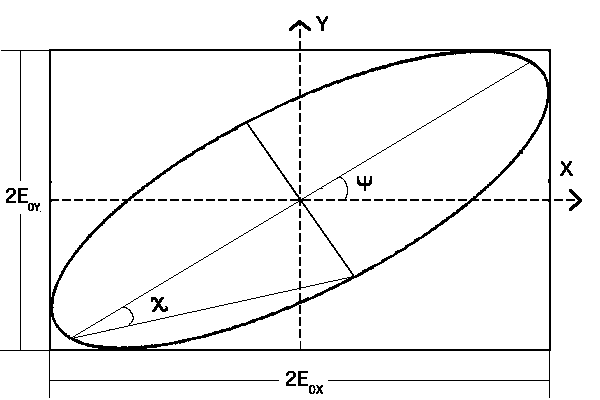
\includegraphics[scale=0.5]{/Sources/Background/Nature_of_Light/polarization-ellipse-binary-v2.png}}
    \end{center}
    \caption{Polarization Ellipse}
    \label{fig:polarization}
\end{figure}
%

Due to the restraints of modern optical sensors, it is not possible to directly measure the polarization ellipse, for a light beam, at any instant in time.  Taking the time average of the ellipse results in quantities that can measured by detectors in order to quantify the polarization state of an EM wave.  It is therefore necessary to derive parameters from the ellipse that can be measured.
Starting from the equation for the polarization ellipse, taking the time average of the E field results in
%
\begin{align}
    \frac{E_x (t)^2}{E_{0x}^2} + \frac{E_y (t)^2}{E_{0y}^2} - \frac{2 E_x (t) E_y (t)}{E_{0x} E_{0y} } cos(\delta)=sin^2 (\delta)
\end{align}
%
the time averages are calculated as [CHECK Fix this equation]
%
\begin{align}
    <E_x (t)^2> = lim_{T \rightarrow \infty} \int_{0}^{2\pi} E_{0x} cos(\tau)  d\tau=\frac{1}{2} E_{0x}^2
\end{align}
%
and similarly
%
\begin{align}
    <E_y (t)^2>  = \frac{1}{2} E_{0y}^2 \\
	<E_x (t) E_y (t)>  =  \frac{1}{2} E_{0x} E_{0y} cos(\delta)
\end{align}
%
substitution into equation and completing the square results in
%
\begin{align}
    (E_{0x}^2+E_{0x}^2 )^2-(E_{0x}^2-E_{0x}^2 )^2-(2E_{0x}^2 E_{0x}^2  cos(\delta) )^2=(2E_{0x} E_{0y}  sin(\delta))^2
\end{align}
%
The terms of this equation represent the polarization state of a wave in relation to the x and y intensities and relative phase delay between the two components.
These quantities are known as the Stokes parameters and describe the state of polarization and are often represented as a vector,
%
\begin{align}
    \vec{S} =
    \begin{bmatrix}
        S_0 \\
        S_1 \\
        S_2 \\
        S_3
    \end{bmatrix}
    =
    \begin{bmatrix}
        E_{0x}^2+E_{0y}^2 \\
        E_{0x}^2-E_{0y}^2 \\
        2E_{0x}^2 E_{0y}^2 cos(\delta) \\
        2E_{0x} E_{0y}  sin(\delta)
    \end{bmatrix}
\end{align}
%
The degree of polarization for an EM wave is the magnitude of the Stokes vector such that
%
\begin{align}
    \alpha =DOP=  \frac{\sqrt{S_1^2+S_2^2+S_3^2 }}{S_0}
\end{align}
%
and ranges from 0 for unpolarized light, to 1 for completely polarized light.  It is possible to show the polarized and unpolarized intensities as individual components
summed together as
%
\begin{align}
    S=S_P+S_U=
    \begin{bmatrix}
        S_0 \\
        S_1 \\
        S_2 \\
        S_3
    \end{bmatrix}
    +(1-DOP)
    \begin{bmatrix}
        1 \\
        0 \\
        0 \\
        0
    \end{bmatrix}
\end{align}
%
The degree of polarization for the linear (DOLP) and circular polarization (DOCP) can specifically be quantified as
%
\begin{align}
    DOLP=  \frac{\sqrt{S_1^2+S_2^2 }}{S_0} \\
    DOCP=  \frac{S_3}{S_0}
\end{align}
%
Note the unpolarized light is represented as
%
\begin{align}
    S=
    \begin{bmatrix}
        S_0 \\
        S_1 \\
        S_2 \\
        S_3
    \end{bmatrix}
    =
    \begin{bmatrix}
        1 \\
        0 \\
        0 \\
        0
    \end{bmatrix}
\end{align}
%
The Stokes parameters can be graphed on a unit sphere, known as the Poincare sphere.  The sphere plots the radial coordinates describing ellipticity and eccentricy of the polarization ellipse as angles of
%
\begin{align}
    Ellipicity = \frac{S_3}{S_0+\sqrt{S_1^2+S_2^2 }}
\end{align}
\begin{align}
    Eccentricity= \sqrt{1-Ellipticity^2}
\end{align}
%
The ellipticity of the polarization ellipse varies from 0, for linearly polarized light, to 1 for purely circular polarization \cite{chipman}.
%
For	graphical representation, Stokes vectors can be plotted on a 3-dimensional sphere known as the Poincare sphere. The sphere is only capable of showing the polarized portion of the EM wave.  Prior to normalization, if the EM wave is not fully polarized, the intensity of the polarized beam must be normalized in relation to the total beam intensity.
%
\begin{figure}[!htb]
    \begin{center}
        \makebox[\textwidth]{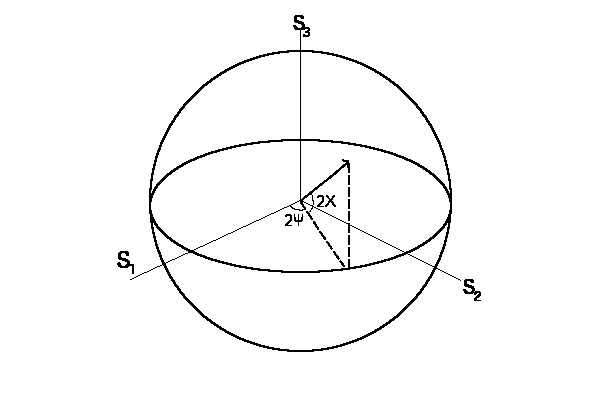
\includegraphics[scale=0.6]{/Sources/Background/Nature_of_Light/POINCARE-binary.png}}
    \end{center}
    \caption{Poincare Sphere}
    \label{fig:polarization}
\end{figure}
%[CHECK]

The zenith angle of the polarization ellipse, represented in Figure as $2\chi$ is found to be related to the parameters of the polarization ellipse by
%
\begin{align}
    sin2\chi = \frac{2E_{0x}2E_{0y}sin\delta}{E_{0x}^2+E_{0y}^2}\qquad -\pi / 4 \leq \chi \leq \pi / 4
\end{align}
%
The azimuth angle $2\psi$ is defined in relation to the parameters of the polarization ellipse as
%
\begin{align}
    tan2\psi = \frac{2E_{0x}2E_{0y}cos\delta}{E_{0x}^2-E_{0y}^2}\qquad 0 \leq \psi \leq \pi
\end{align}
%
For a given state of the polarization ellipse, the angles for plotting the corresponding polarization state on the Poincare sphere can be found using these equations\cite{spieellipse}.

%%%%%%%%%%%%%%%%%%%%%%%%%%%%%%%%%%%%%%%%%%%%%%%%%%%%%%%%%%%
\subsection{Jones Vector Representation}
%%%%%%%%%%%%%%%%%%%%%%%%%%%%%%%%%%%%%%%%%%%%%%%%%%%%%%%%%%%
    %need subsub section on Jones
    % need subsub section on Devices
For the special case of fully polarized EM waves, DOP = 1, the polarization of the beam can be described by a 2x 1 complex vector known as a Jones vector.  The Jones vector relies on the fact that the polarization state of a beam depends only on its relative $X$ and $Y$ intensities, as well as the phase delay between each respective component.

Converting the equation for the electric component of the EM wave into a phasor makes it easy to see the parameters that determine the beam's polarization.  A phasor represents a sinusoidal wave with a constant frequency.  The Jones vectors can be formulated from this representation as
%
\begin{align}
    \underline{\hat{E}}(z)=(\vec{i_x} E_{0x} e^{j\delta_x}+\vec{i_y} E_{0y} e^{j\delta_y })e^{-kz}
\end{align}
%
since the polarization depends on the amplitude and phase difference of the $X$ and $Y$ components, the Jones vector is formally written as
%
\begin{align}
    \underline{J} =
    \begin{bmatrix}
        E_{0x} e^{j\delta_x} \\
        E_{0y} e^{j\delta_y }
    \end{bmatrix}
\end{align}
%
Since only the relative phase differences matter it is common to denote $\delta=\delta_y-\delta_x$.  The vector is also normalized by dividing by its magnitude,
%
\begin{align}
    \underline{J} =
    \frac{1}{\sqrt{E_{0x}^2 + E_{0y}^2}}
    \begin{bmatrix}
        E_{0x} e^{j\delta_x} \\
        E_{0y} e^{j\delta_y }
    \end{bmatrix}
\end{align}
%
An angle can then be defined such that
%
\begin{align}
    tan(\psi) = \frac{E_{0y}}{E_{0x}}
\end{align}
%
The Jones vector can then be written in terms of a single angle
%
\begin{align}
    \underline{J_{\delta}}(\psi) =
    \begin{bmatrix}
        cos(\psi) \\
        sin(\psi)e^{j\delta}
    \end{bmatrix}
\end{align}
%
General states of linear polarization are represented as
%
\begin{align}
    \underline{J_0}(\psi) =
    \begin{bmatrix}
        cos(\psi) \\
        sin(\psi)
    \end{bmatrix}
\end{align}
%
where $\psi$ is any angle in relation to the X axis.  Circular polarization is represented as
%
\begin{align}
    RCP: \underline{J}_{\frac{\pi}{2}} = \frac{1}{\sqrt{2}}
    \begin{bmatrix}
        1 \\
        j
    \end{bmatrix} \\
    LCP: \underline{J}_{-\frac{\pi}{2}} = \frac{1}{\sqrt{2}}
    \begin{bmatrix}
        1 \\
        -j
    \end{bmatrix}
\end{align}
%
\subsubsection{Optical Devices}
Polarization can be naturally occurring, such as in the case of skylight, or it can be created by passing light through an optical device such as a linear polarizer or a quarter wave plate.  Jones vectors are useful for describing the polarization state of an EM wave, while Jones matrices describe nondepolarizing optical devices and the transformation of pure incident polarization states through them.

A linear polarizer is a device that transmits linear polarization states for incident light beams that are aligned with their transmission axis (TA) of the polarizer \cite{polarizedlight}.  For example, if horizontally polarized light is passed through a polarizer with a $TA = 90^{\circ}$, all of the incident light will be extinguished.  In practice all of the light is not completely extinguished and there are often spectral differences to the response of polarizers.

Since linear polarizers block light that is orthogonal to the TA, it can be shown that the general equation for a linear polarizer is such that
%
\begin{align}
    \underline{J}_{in}(\psi + \frac{\pi}{2}) =
    \begin{pmatrix}
        cos(\psi + \frac{pi}{2}) \\
        sin(\psi + \frac{pi}{2})
    \end{pmatrix}
    =
    \begin{pmatrix}
        -sin(\psi) \\
        cos(\psi)
    \end{pmatrix}
\end{align}
%
and
\begin{align}
    \underline{J}_{out} =
    \begin{pmatrix}
        0 \\
        0
    \end{pmatrix}
\end{align}
%
The general equation for Jones interaction with a linear polarizer is
%
\begin{align}
    P(\psi)\underline{J}_{in} = \underline{J}_{out}
\end{align}
\begin{align}
    \begin{pmatrix}
        a & b \\
        c & d
    \end{pmatrix}
    \begin{pmatrix}
        -sin(\psi) \\
        cos(\psi)
    \end{pmatrix}
    =
    \begin{pmatrix}
        0 \\
        0
    \end{pmatrix}
\end{align}
\begin{align}
    -asin(\psi) + bcos(\psi) = 0 \rightarrow atan(\psi) \\
    -csin(\psi) = dcos(\psi) = 0 \rightarrow ctan(\psi)
\end{align}
%
When the incident polarization state is aligned with the polarizers TA, it must also be true that the incident beam goes through the device unchanged.  Therefore,
%
\begin{align}
    \underline{J}_{in}(\psi) =
    \begin{pmatrix}
        cos(\psi) \\
        sin(\psi)
    \end{pmatrix} \\
    \underline{J}_{out}(\psi) =
    \begin{pmatrix}
        cos(\psi) \\
        sin(\psi)
    \end{pmatrix}
\end{align}
\begin{align}
    acos(\psi) + bsin(\psi) = cos(\psi) \\
    ccos(\psi) + dsin(\psi) = sin(\psi)
\end{align}
%
substituting in for previous values of b and d give
%
\begin{align}
    a = \frac{cos(\psi)}{cos(\psi) + tan(\psi)sin(\psi)} = cos^2\psi
\end{align}
\begin{align}
    b = atan(\psi) = sin(\psi)cos(\psi)
\end{align}
\begin{align}
    c = \frac{sin(\psi)}{cos(\psi) + tan(\psi)sin(\psi)} = sin(\psi)cos(\psi)
\end{align}
\begin{align}
    d = ctan(\psi) = sin^2\psi
\end{align}
%
The general form of a linear polarizer with transmission axis angle ? from the X axis is
%
\begin{align}
    P(\psi) =
    \begin{pmatrix}
        cos^2\psi & sin(\psi)cos(\psi) \\
        sin(\psi)cos(\psi) & sin^2\psi
    \end{pmatrix}
\end{align}
%
The intensity of light emerging from a polarizer is governed by Malus law,
%
\begin{align}
    I = I_0cos^2(\theta_i)
\end{align}
%
where $I$ is the intensity of the exiting beam, $I_0$ is the intensity of the incident beam and $\theta_i$ is the angle between the incident polarization state, and the angle of the polarizer.   For incident unpolarized light the equation becomes $I / I_0 = \frac{1}{2}$.  Therefore, the maximum transmittance for an unpolarized beam of light through a polarizer is 50%.  This number is significantly lower for polaroid film based polarizers and can cause potential problems with detector sensitivity for low lighting conditions.

Wave plates create a phase delay between the fast and slow axis of incident linearly polarized light.  Its generalized Jones matrix form can be denoted with a relative phase delay $\delta=\delta_y-\delta_x$,
\begin{align}
    C(\delta) =
    \begin{pmatrix}
        1 & 0 \\
        0 & e^{-j\delta}
    \end{pmatrix}
\end{align}
%
Two common wave plates are the half wave plate and the quarter wave plate.  These produce a delay of $\pi$ and $\pi/2$ respectively.

The noobelectric python package has a module for dealing with these types of problems and it automates Jones optical calculations for purely polarized light beams.  An example for a linear polarizer combined with a quarter wave plate can be created and various input polarization states into the system as shown below.
\begin{lstlisting}
>>> from noobee.jones import j, lp
>>> j_in = j(1,0)
>>> lp_1 = lp(0)
>>> lp_1 * j_in
matrix([[ 1.],
        [ 0.]])
\end{lstlisting}

%%%%%%%%%%%%%%%%%%%%%%%%%%%%%%%%%%%%%%%%%%%%%%%%%%%%%%%%%%%
\subsection{Mueller Matrices}
%%%%%%%%%%%%%%%%%%%%%%%%%%%%%%%%%%%%%%%%%%%%%%%%%%%%%%%%%%%
Interactions with materials that can create depolarization and model partially polarized input and outputs cannot be handled by Jones calculus.  For these problems, Mueller Matrices are used to model the polarization of light with varying degrees of polarization as it interacts with a material.  These interactions are modeled with the equation
\begin{align}
    \mathbf{S}_{out} = \mathbf{M}\mathbf{S}_{in}
\end{align}
%
where
%
\begin{align}
    \mathbf{M} =
    \begin{bmatrix}
        m_{00} & m_{01} & m_{02} & m_{03} \\
        m_{10} & m_{11} & m_{12} & m_{13} \\
        m_{20} & m_{21} & m_{22} & m_{23} \\
        m_{30} & m_{31} & m_{32} & m_{33} \\
    \end{bmatrix}
\end{align}
%
is 4x4 Mueller Matrix that describes the diattenuation, depolarization, and retardance of a materials' polarization response to an input EM beam.

Diattenuation – the two attenuations of orthogonal polarization states [7]

Retardance – the phase difference between two orthogonal polarization states [8]

Depolarization – a process where polarized light becomes unpolarized [8]

It has been shown that these parameters can be found by determining a sample's corresponding Mueller Matrix. The scalar parameters are mathematically defined as,
\begin{align}
    %\emphasis{Diattenuation} = \frac{\sqrt{m_{01}^2 + m_{02}^2 + m_{03}^2}}{m_{00}} \\
%    \emphasis{Retardance} = cos^{-1}(\frac{tr(M_{ret})}{2}-1) \\
%    \emphasis{Depolarization} = 1 - \frac{\sqrt{\sum_{i,j}m_{ij}^2} -m_{00}^2}{\sqrt{3}m_{00}^2}
\end{align}
[TODO explain these equations or remove them]

For nondepolarizing materials, their MM can be converted into Jones matrices.   Examples of Mueller Matrices for common optical elements can be found in [7].  The general form of a linear polarizer with transmission axis at 0 degrees to the $x$ axis is
%
\begin{align}
    \mathbf{M} =
    \begin{bmatrix}
        q + r & q - r & 0 & 0 \\
        q-r & q+r & 0  & 0 \\
        0 & 0 & 2\sqrt{qr} & 0 \\
        0 & 0 & 0 & 2\sqrt{qr}
    \end{bmatrix}
\end{align}
%
where q and r are the attenuation coefficients for the X and Y axis.

%%%%%%%%%%%%%%%%%%%%%%%%%%%%%%%%%%%%%%%%%%%%%%%%%%%%%%
\subsubsection{Mueller Matrix Decomposition}
%%%%%%%%%%%%%%%%%%%%%%%%%%%%%%%%%%%%%%%%%%%%%%%%%%%%%%

The effects of diattenuation, depolarization and retardance can be found to be represented as subsets of the Muller matrix through its decomposition such that the result is
\begin{align}
    \mathbf{M} = m_{00}
    \begin{bmatrix}
        1 & \mathbf{D}^T \\
        \mathbf{P} & \mathbf{m}
    \end{bmatrix}
\end{align}
The derivation of the MM decomposition was made known by Lu and Chipman and is reproduced in [14]. $\mathbf{D}^T$ is the diattenutation vector that describes the amount of decrease in overall polarization for each set of orthogonal polarization states. The m matrix represents the retardance of a material.

$\mathbf{P}$ is the polarizance vector, and describes the amount of light that becomes polarized when unpolarized light is incident.  It is analogous to the effect of depolarization.  This vector can be measured by detecting the output Stokes vector of a material when unpolarized light is incident.  This effect is only evident in materials that create polarization.

%%%%%%%%%%%%%%%%%%%%%%%%%%%%%%%%%%%%%%%%%%%%%%%%%%%%%%%%%%%
\subsection{Reflection and Transmission}
%%%%%%%%%%%%%%%%%%%%%%%%%%%%%%%%%%%%%%%%%%%%%%%%%%%%%%%%%%%

When light interacts with two materials that have different indexes of refraction, the incident beam is reflected and transmitted according to Fresnel’s equations.

The law of reflection states
%
\begin{align}
    \theta_i = \theta_r
\end{align}
%
The transmission is derived directly from Snells equation,
%
\begin{align}
    n_1sin(\theta_i) = n_2sin(\theta_2)
\end{align}
%
Note that part of the transmitted spectra may be absorbed, although this is not considered in these equations.

Two main scenarios are often presented when demonstrating the principles which guide the reflected and transmitted rays; when the incident electromagnetic wave is polarized perpendicular to the plane of incidence, and when the wave is polarized parallel to it.  The perpendicular polarized wave is often denoted S or TE for transverse electric, while the parallel scenario is often denoted P or TM for transverse magnetic.

\begin{figure}[!htb]
    \begin{center}
        \makebox[\textwidth]{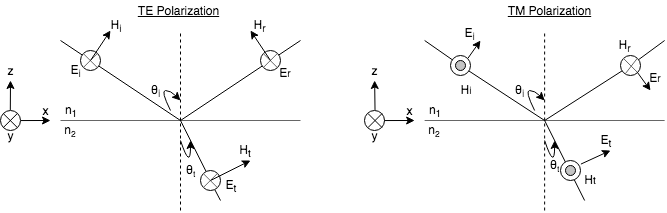
\includegraphics[scale=0.6]{/Sources/Background/Nature_of_Light/fresnel-reflect-trans.png}}
    \end{center}
    \caption{Fresnel Reflection and Transmittance}
    \label{fig:polarization}
\end{figure}

The intensity of the reflected waves for the S and P polarized case are
%
\begin{align}
    \mathbf{R_S} = |\frac{Z_2cos(\theta_i)-Z_1cos(\theta_t)}{Z_2cos(\theta_i)+Z_1cos(\theta_t)}|^2
\end{align}
\begin{align}
    \mathbf{R_P} = |\frac{Z_2cos(\theta_t)-Z_1cos(\theta_i)}{Z_2cos(\theta_t)+Z_1cos(\theta_i)}|^2
\end{align}
%
where Z is the wave impedance for medium 1 and 2.  The power coefficients for transmission are then derived by following the law of conservation of energy such that,
%
\begin{align}
    T_S = 1 - R_S \\
    T_P = 1 - R_P
\end{align}
%
The Brewster angle is a special case where the $P$ polarization state is completely transmitted and no reflection of the TM wave occurs.  The reflected ray is therefore completely $S$ polarized since $R_P$ is zero and $R_S$ is a nonzero intensity.  For perfect air glass interactions typically considered, this angle is approximately 55 degrees.

The Mueller matrix formulation for reflection and transmission reduces to the form of a linear polarizer for ideal surfaces.  It has been shown in \cite{polarizedlight} that the equation for a reflected beam off of a perfectly smooth dielectric surface is
%
\begin{align}
    \begin{split}
    \begin{bmatrix}
        S_{0r} \\
        S_{1r} \\
        S_{2r} \\
        S_{3r}
    \end{bmatrix}
    =
    \frac{1}{2}(\frac{tan(\theta_{-})}{sin(\theta_{+})})^2
    \begin{bmatrix}
       p_S^2 + p_P^2 & p_S^2 - p_P^2 & 0 & 0 \\
        p_S^2 - p_P^2 & p_S^2 + p_P^2 & 0 & 0 \\
        0 & 0 & 2p_Sp_P & 0 \\
        0 & 0 & 0 & 2p_Sp_P
    \end{bmatrix}
    \begin{bmatrix}
        S_0 \\
        S_1 \\
        S_2 \\
        S_3
    \end{bmatrix}
    \end{split}
\end{align}
%
\begin{align}
    p_S = cos^2(\theta_{-}) \\
    p_P = cos^2(\theta_{+})
\end{align}
and $\theta_{\pm}=\theta_i \pm \theta_r$.
This is identical to the form of a linear diattenuator or polarizer from Equation 2.60. For incident unpolarized light the equation simplifies to
%
\begin{align}
    \begin{bmatrix}
        S_{0r} \\
        S_{1r} \\
        S_{2r} \\
        S_{3r}
    \end{bmatrix}
    =
    \frac{1}{2}(\frac{tan(\theta_{-})}{sin(\theta_{+})})^2
    \begin{bmatrix}
        cos^2(\theta_{-}) + cos^2(\theta_{+}) \\
        cos^2(\theta_{-}) - cos^2(\theta_{+}) \\
        0 \\
        0
    \end{bmatrix}
    S_0
\end{align}
%
Therefore, for ideal reflective surfaces, at the Brewster angle, light will be completely polarized perpendicular to the plane of incidence. It should be noted that the case of incident unpolarized light onto the target material, gives the polarizance vector of the Mueller Matrix as described in Section 2.1.3.

Imperfect, non-ideal surfaces have the ability to reflect, transmit and absorb incident electromagnetic radiation.  The outcome of these interactions are related to the physiological makeup of the material, as well as its surface topology.  Multiple scattering mechanisms can be at work within a system, and numerous models have been attempted to balance the tradeoffs between practical realizability for measurements and accurate representation of scattering mechanisms \cite{priest}, \cite{pbrdf}.  Only some of these models attempt to deal with the polarization of the incident, reflected, and transmitted beams.

%%%%%%%%%%%%%%%%%%%%%%%%%%%%%%%%%%%%%%%%%%%%%%%%%%%%%%%%%%%
\subsection{Scattering Mechanisms}
%%%%%%%%%%%%%%%%%%%%%%%%%%%%%%%%%%%%%%%%%%%%%%%%%%%%%%%%%%%

Fresnel’s equations provide an explanation for light reflected and transmitted for ideal surfaces.  This is not the case with most man made and natural materials.  Therefore, more complex mechanisms must be considered when dealing with real world radiation scattering problems.  It has become popular in the field of remote sensing to denote the additional types of interactions as volume scattering and multiple scattering
 interaction.  Single scattering mechanisms are those governed solely by Fresnel’s equations.  The combination of these scattering mechanisms create the diffuse and specular components of reflection.

Single scattering mechanisms create a portion of reflectance known as specular reflectance.  They are often denoted as Type A photons in remote sensing models.  These interactions are highly polarized perpendicular to the plane of incidence as previously discussed. For perfectly smooth dielectrics, this is the dominant scattering mechanism.

Volume scattering occurs when light is absorbed by a material and is readmitted in all directions, including back towards the surface of the material.  They are denoted Type B photons.  Transmittance of this energy back into the first medium obeys the laws of Fresnel’s equations, although the indices of refraction are reversed.  This mechanism accounts for absorption and other higher level light matter interactions, not explained solely by Fresnel’s equations.

Multiple scattering occurs when either Type A or Type B photons interact with the material surface more than once while either being reflected or retransmitted out of the material.  These are denoted Type C photons \cite{schott}.  Figure 2.7 shows each type of interaction.
%
\begin{figure}
    \begin{center}
        \makebox[\textwidth]{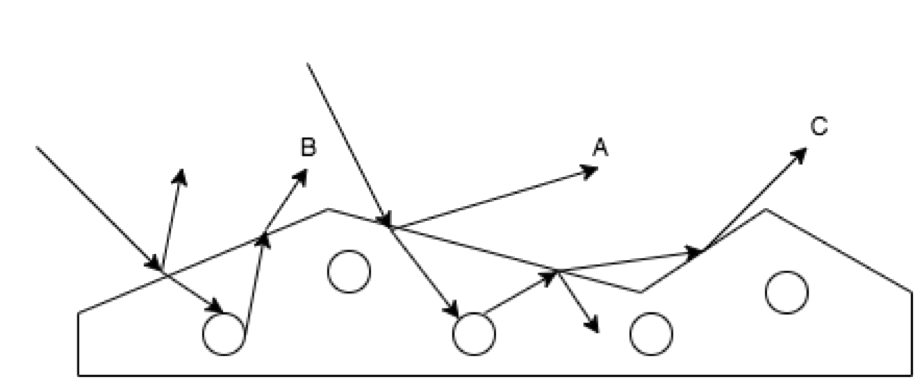
\includegraphics[scale=0.75]{/Sources/Background/Nature_of_Light/photon-interactions-wo.png}}
    \end{center}
    \caption{Various Types of Photon Interactions}
    \label{fig:scattering}
\end{figure}
%
In general type A photons create specular highlights from surfaces that are smooth.  Type B and C photons become more prevalent as a surface becomes rougher.  In most real world applications, surfaces are neither purely specular nor purely diffuse.

Surfaces that are perfectly smooth dielectrics are often considered to be purely specular reflectors of light.  Incident energy is transmitted in an idealized single ray of light from the surface.  Specular reflectors are single scattering mechanisms and result in purely polarized light due to the governance of Fresnel’s equations and are denoted as type A photons.
%
\begin{figure}
    \begin{center}
        \makebox[\textwidth]{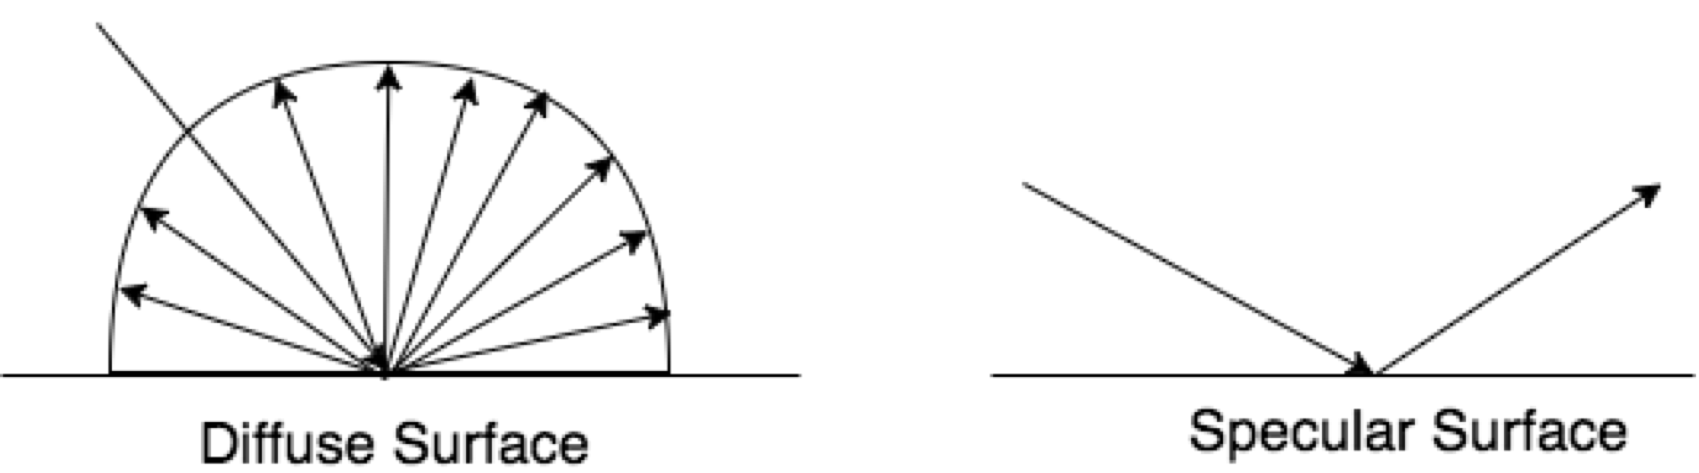
\includegraphics[scale=0.45]{/Sources/Background/Nature_of_Light/diffuse-specular.png}}
    \end{center}
    \caption{Diffuse and Specular Scattering}
    \label{fig:scattering}
\end{figure}
%
In simple models, rough surfaces can be viewed as purely diffuse reflectors that scatter incident light equally in all directions.  Figure 2.8 shows a general example of both specular and diffuse surface scattering.  Perfect diffuse surfaces are known as Lambertian surfaces.  It has been assumed that the diffuse portion of light is unpolarized due to random nature of internal reflections \cite{specularclass}, \cite{grant}.
\begin{figure}
    \begin{center}
        \makebox[\textwidth]{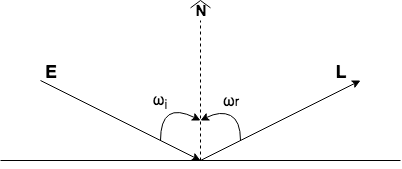
\includegraphics[scale=0.7]{/Sources/Background/Nature_of_Light/brdf-simple.png}}
    \end{center}
    \caption{Simple BRDF Model}
    \label{fig:scattering}
\end{figure}
Bidirectional Reflectance Distribution Functions (BRDF) have been created to model the variety of surface interactions in order to handle the nonideal case where surface roughness is present. BRDFs define how incident radiation is reflected off of opaque surfaces.  It is defined as a ratio of reflected radiance along path $\omega_r$ to incident irradiance $\omega_i$. A simple depiction of this scenario can be found in Figure 2.9.

The BRDF function is often defined in the form
%
\begin{align}
    f_r(\omega_i, \omega_r) = \frac{dL_r(\omega_r)}{dE_i(\omega_i)}[{sr}^{-1}]
\end{align}
%
The units of the BRDF can be reduced from
\begin{align}
    [\frac{dL_r(\omega_r) units}{dE_i(\omega_i) units}] = [\frac{\frac{W}{m^2sr}}{\frac{W}{m^2}}] = [\frac{1}{sr}] = [{sr}^{-1}]
\end{align}
Each $\omega$ is a function of azimuth angle $\phi$ and zenith angle $\theta$. The input irradiance $E$ and output radiance $L$ are measured in units of watts per meter squared and watts per meter squared steradians as shown in Figure 2.10.
where numerous models have been developed for the functions of $L$ and $E$ \cite{sparrow}\cite{brdfoverview}.  In its simplest case the surface is a purely diffuse reflector of incident light and the BRDF becomes
%
\begin{align}
    f_r(\omega_i, \omega_r) = \frac{\rho}{\pi}[{sr}^{-1}]
\end{align}
%
where $\rho$ is the surface albedo, or proportion of light reflected from a surface \cite{nicodemus} and ranges from $0\leq\rho\leq1$.  A general diagram can be found in Figure 2.9.  In the most general case the portion of reflectance that is purely specular can be thought of as a $\delta$ function.  Most surfaces create non-ideal reflections made up of both specular and diffuse components.
%
\begin{figure}
    \begin{center}
        \makebox[\textwidth]{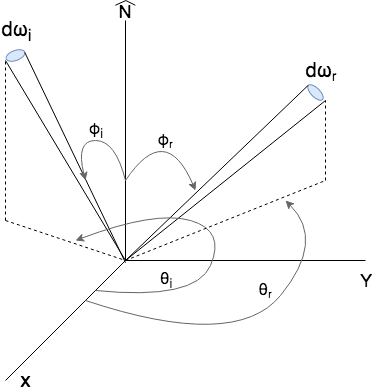
\includegraphics[scale=0.7]{/Sources/Background/Nature_of_Light/brdf-v2.png}}
    \end{center}
    \caption{General BRDF Model}
    \label{fig:scattering}
\end{figure}
%
The notion of a surface being rough, smooth, fine or coarse has been discussed from a perspective of polarized scattering mechanisms. These surface descriptions also come with a connotation of touch and the feel of a materials' surface.  They are textures.


%%%%%%%%%%%%%%%%%%%%%%%%%%%%%%%%%%%%%%%%%%%
\section{Texture and Tone}
%%%%%%%%%%%%%%%%%%%%%%%%%%%%%%%%%%%%%%%%%%%

“When small image areas from black and white photographs are independently processed by a machine, then texture and tone are most important” [4].  Without tone there is no texture, as texture is created when there are certain frequencies of tonal change in an image [12].

A surface texture is classified according to the scale at which the human eye can see.  It is import to determine the appropriate scale for a particular surface, when talking about its texture.  A surfaces ability to appear smooth or rough in an image, is determined by the spatial frequency distribution of grey level pixel intensities in a greyscale image and the various shades of grey tones.  The nature of light reflecting from surfaces of materials is also largely due to the how rough or smooth the surface is.  Imaging devices are able to pick up pixel by pixel surface interactions in their large field of view.  Cameras are able to detect multiple scattering mechanisms for analysis in material classification problems.

Tone is related to texture and is the grey level gradients distributed across an image.  It is the “relative brightness or color of objects on an image” [12].  If an image has no differences in tone, then the texture and other features are indiscernible.

When a pixel is considered as a single color receptor, it represents only tone.  The scaling of the window size to include more pixels allows for texture to become more prevalent.   Scale is important when considering texture since texture is defined in relation to our perception of a materials surface.


%%%%%%%%%%%%%%%%%%%%%%%%%%%%%%%%%%%%%%%%%%%
\subsection{Grey Level Co-Occurence Matrix}
%%%%%%%%%%%%%%%%%%%%%%%%%%%%%%%%%%%%%%%%%%%
A Grey Level Co-Occurrence Matrix (GLCM) is able to quantify the spatial frequency distribution of grey level pixel intensity pairs. The GLCM matrix is formed by determining the frequency of grey level value pixel pairs for a given image.  A relationship is set a priori to determine the direction for grey level comparison.  This relationship is an angle relating a pixel to its neighbor, and is chosen in multiples of either 0 or 45 degrees.  Common GLCM spatial relationships are $0, \pi/4, 3\pi/4, and \pi/2$ radians.
%
\begin{figure}[!htb]
    \begin{center}
        \makebox[\textwidth]{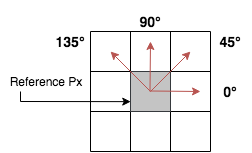
\includegraphics[scale=0.75]{/Sources/Background/Texture_and_Tone/glcm-relationships-no-title.png}}
    \end{center}
    \caption{Defining GLCM Relationships}
    \label{fig:texture}
\end{figure}
%
In order to quantify a texture in a rotationally consistent fashion, all four relationships are usually calculated and averaged together in determining the overall GLCM matrix.  The GLCM has a size of $N x N$ where $N$ is the discrete quantized levels.

A single relationship Co-Occurence matrix is formulated such that,
%
\begin{align}
    \mathbf{\phi}_{ij}(\triangle x,\triangle y) = \sum_{x=0}^{n}\sum_{y=0}^{m}
    \begin{cases}
        1, if I(x,y) = i  and  I(x+\triangle x,y+\triangle y) = j \\
        0, otherwise
    \end{cases}
\end{align}
%
where $I(x,y)$ is an $n x m$ image and $\triangle x,\triangle y$ represent the predefined offset of the grey level pixel neighbor intensity relationship (i,j).
Being defined as referencing one pixel to its neighbor to the right (0 degrees) the GLCM matrix is formulated as such,
%
\begin{figure}[!htb]
    \begin{center}
        \makebox[\textwidth]{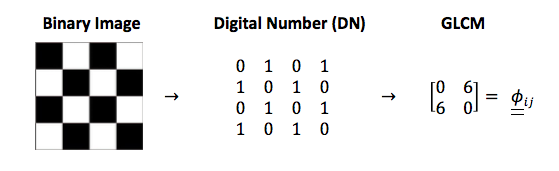
\includegraphics[scale=0.75]{/Sources/Background/Texture_and_Tone/glcm.png}}
    \end{center}
    \caption{Converting a Binary Image to a GLCM Matrix}
    \label{fig:texture}
\end{figure}
%[CHECK]
The example in Figure 2.6 shows the simplest case of a binary image, or an image that only contains white and black pixels.  These pixels values captured by a camera are then converted into there corresponding digital numbers, in this case either zero or one.  With the spatial relationship being defined as one to the right, the GLCM matrix is then formed.

Non symmetrical GLCMs should be symmetrized by adding each to its transpose,
%
\begin{align}
    \mathbf{\phi}^{'} = \mathbf{\phi} + \mathbf{\phi}^{T}
\end{align}
%
Normalizing the frequency to one by dividing the matrix by the sum of all its elements, results in a probability distribution for each grey level pixel pair.
%
\begin{align}
    \mathbf{P} = \frac{\mathbf{\phi}^{'}}{\sum_{i=0}^{N-1}\sum_{j=0}^{N-1}\mathbf{\phi}^{'}}
\end{align}
%
where for the example given above the resulting $\mathbf{P}$ is
%
\begin{align}
    \mathbf{P} = \frac{1}{12}
    \begin{bmatrix}
        0 & 6 \\
        6 & 0
    \end{bmatrix}
    =
    \begin{bmatrix}
        0 & 0.5 \\
        0.5 & 0
    \end{bmatrix}
\end{align}
%
As expected the probability of finding a 0 next to a 1 is the same as finding a 1 next to a zero in a binary checkerboard image.

Features can then be extracted from the formed matrix for the purpose of defining single quantitative values for texture.  These features are known as Haralick features and generally fall into 3 distinct feature categories; Contrast, Statistical and measures of Orderliness \cite{calgary}.

Contrast measures are defined by weights that increase or decrease with distance from the GLCM diagonal.  These weights can be linear, exponential, etc. For the N x N dimensional GLCM matrix the N - 1 term in the first row or column represents pixel relationships that are of the greatest intensity difference.

For example, an 8-bit image has 256 possible grey level values ranging from 0-255, so the maximum amount of contrast occurs when pixel pairs (i,j) are either (0, 255) or (255, 0).

Contrast has weights that increase exponentially away from the diagonal.  It is calculated as
%
\begin{align}
    Contrast = \sum_{i=0}^{N-1}\sum_{j=0}^{N-1}(i-j)^2P_{ij}
\end{align}
%
The dissimilarity is a measure of contrast with weights that increase linearly away from the diagonal
%
\begin{align}
    Diss = \sum_{i=0}^{N-1}\sum_{j=0}^{N-1}|i-j|P_{ij}
\end{align}
%
The dissimilarity of the example binary image can be calculated as
%
\begin{align}
    Diss = \sum_{i=0}^{N-1}\sum_{j=0}^{N-1}|i-j|P_{ij}
    = \sum_{1=0}^{1}|i|P_{i0}+|i-1|P_{i1}
    = 0 + P_{01} + 0 + P_{10} = \frac{1}{3}
\end{align}
%
Statistical measures utilize each individual element of the GLCM as weights to determine the moments of the probability distribution matrix. The mean, variance, correlation, etc. are not measures of individual pixel intensity values, but rather of the intensity of a pixel in relation to its neighbor’s intensity. The mean is the first central moment and is defined by
%
\begin{align}
    \mu_i = \sum_{i=0}^{N-1}\sum_{j=0}^{N-1}iP_{ij} \\
    \mu_j = \sum_{i=0}^{N-1}\sum_{j=0}^{N-1}jP_{ij}
\end{align}
%
Variance is the second moment of the GLCM and is defined as,
%
\begin{align}
    \sigma_i = \sum_{i=0}^{N-1}\sum_{j=0}^{N-1}(i-\mu_i)^2P_{ij}
\end{align}
\begin{align}
    \sigma_j = \sum_{i=0}^{N-1}\sum_{j=0}^{N-1}(j-\mu_j)^2P_{ij}
\end{align}
%
The correlation shows the “linear dependency of grey level values in the Co-Occurence matrix”\cite{haralickcancer}.  It is computed from the values of the variance and mean such that
%
\begin{align}
    Corr = \sum_{i=0}^{N-1}\sum_{j=0}^{N-1}(\frac{(i-\mu_i)(j-\mu_j)}{\sqrt{\sigma_i^2 \sigma_j^2}})
\end{align}
%
If a the GLCM is symmetric, the x and y means and variances are equal and the equations simplify to,
%
\begin{align}
    \mu = \sum_{i=0}^{N-1}\sum_{j=0}^{N-1}iP_{ij}
\end{align}
\begin{align}
    \sigma = \sum_{i=0}^{N-1}\sum_{j=0}^{N-1}(i-\mu)^2P_{ij}
\end{align}
\begin{align}
    Corr = \sum_{i=0}^{N-1}\sum_{j=0}^{N-1}(\frac{(i-\mu)(j-\mu)}{\sigma^2})
\end{align}
%
Measures of orderliness are quantified by the amount of entropy and energy within an image.  Entropy is a measure of randomness in a system.  In thermodynamics, it is the heat lost when a reaction occurs and hence is a measure of disorder.  Energy is a measure of useful work that can occur due to the non random nature of the energy in a system. (clean up this bit on entropy)

The angular second moment (ASM) describes the amount of “inertia” around a pixel neighbor relationship and is defined as,
%
\begin{align}
    ASM = \sum_{i=0}^{N-1}\sum_{j=0}^{N-1}P_{ij}^2
\end{align}
%
The square root of the ASM results in the energy of the system
%
\begin{align}
    Energy = \sqrt{ASM}
\end{align}
%
For perfectly uniform textures the energy will be at a maximum of 1.


%%%%%%%%%%%%%%%%%%%%%%%%%%%%%%%%%%%%%%%%%%%
\section{Plant Physiology}
%%%%%%%%%%%%%%%%%%%%%%%%%%%%%%%%%%%%%%%%%%%
A plant's health is greatly determined by the availability of light, water, and key nutrients in the soil.  These elements are the fundamental inputs to photosynthesis, the process plants utilize to turn light energy into chemical energy for growth.  Nitrogen, Potassium, and Phosphorus are fertilizers (agricultural inputs) that can incur large costs when applied over hectares of farmland, but are needed for healthy plant growth and cell reproduction.

Water is also an essential agricultural input needed for plant photosynthesis and aids in nutrient transport.  Droughts are becoming a global epidemic and precision water management is becoming pivotal for a crops' survival.

The layers of a deciduous leaf contain protection mechanisms, transport systems, and reaction centers for the process of photosynthesis.

%[CHECK insert image of plant layers]
\begin{figure}[!htb]
    \begin{center}
        \makebox[\textwidth]{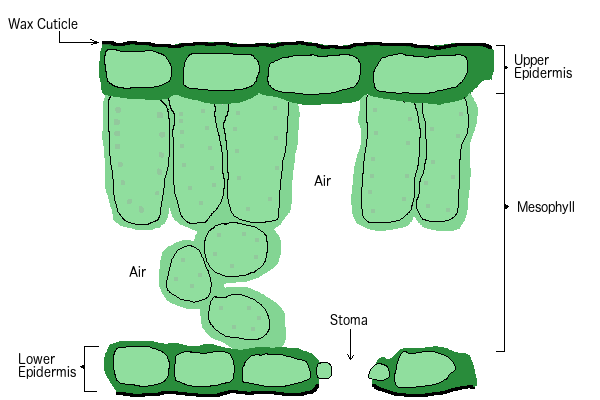
\includegraphics[scale=0.5]{/Sources/Background/Plant_Physiology/leaf-v3.png}}
    \end{center}
    \caption{Major Structures of a Leaf}
    \label{fig:polarization}
\end{figure}

The cuticle wax layer, upper epidermis, and mesophyll layer are the first layers of light interaction on the adaxial surface of the leaf.

The cuticle wax layer provides “the most critical adaptive trait for survival … the ability to retain water in increasingly dehydrating habitats” \cite{cuticle}.  It is the first line of defense for plants and acts as a barrier between water transpiration.

The mesophyll layers contain chloroplasts that convert light energy into chemical energy and consists of two parts. The palisade mesophyll is made up of elongated, organized, compact cells that contain a large number of the chloroplasts.  The spongy mesophyll is irregular in shape and has a large amount of space between its cells to facilitate air and gas exchange [TODO find source].

The upper epidermis consists of very few chloroplasts, and allows most of the light to pass through to the mesophyll layers.


%%%%%%%%%%%%%%%%%%%%%%%%%%%%%%%%%%%%%%%%%%%
\subsection{Photosynthesis}
%%%%%%%%%%%%%%%%%%%%%%%%%%%%%%%%%%%%%%%%%%%

Photosynthesis is a fundamental process that dictates the growth of all land plants.  Water plays an important role in this chemical process, and its availability in plant leaves is an indicator of the plant's ability to perform photosynthesis.

The chemical reaction undergone during photosynthesis involves the conversion of carbon dioxide and water with light energy, to create a carbohydrate and oxygen.  It is formally written as,
%
\begin{align}
    6CO_2 + 6H_2O \xrightarrow{\text{light}} C_6H_12O_6 + 6O_2
\end{align}
%
Due to water's integral role in this reaction, water stress in plants can lead to decreased photosynthetic activity.  It was pointed out by Ehleringer, referenced in \cite{akinci}, that water stress “can decrease…photosynthesis by reflecting quanta that might have been used in photosynthesis”.   Chlorophyll is an essential pigment in photosynthesis due to it being “an efficient light-absorbing molecule” \cite{ecophysiology}.  It is highly absorbing in the blue and red spectrum of visible light, and more reflective in the green portion.  The absorption spectrum for chlorophyll can be found in \cite{chemistry}. This spectrum is what causes many leaves to appear green.  Note that is regions outside the visible, chlorophyll does not absorb the incident radiation.

%%%%%%%%%%%%%%%%%%%%%%%%%%%%%%%%%%%%%%%%%%%
\subsection{Relative Water Content}
%%%%%%%%%%%%%%%%%%%%%%%%%%%%%%%%%%%%%%%%%%%
The Relative Water Content (RWC) of a leaf is a measure of the current water level based on the total leaf water retaining capacity.  It is a useful measure of the water balance within a plant as it expresses the absolute amount of current water in a plant, in proportion to the minimum amount of water it can hold.

Water makes up over 90\% of the mass of a leaf, and although RWC provides a good indicator of plant health and water capacity, it is highly dependent on the age and maturity of the leaf.  It should also be taken into consideration that leaves can also be very heterogeneous and contain a variety of complex structures in different stages of growth, within each individual leaf.

Correlations between the RWC and other physiological responses have been found in [9].

\begin{table}[h]
  \centering
  \begin{tabular}{ll}
    \toprule
    \textbf{Relative Water Content ~(\%)}      & \textbf{Plant Physiological Response}\\
    \midrule
      \texttt{90-100}          & closing of the stomata, reduction of cellular expansion and growth\\
      \texttt{80-90}           & tissue composition change, altered rates of photosynthesis and respiration\\
      \texttt{<80}         & ceasing of photosynthesis\\
    \bottomrule
  \end{tabular}
  \caption{%
    Plant physiological responses to detected relative water content levels.
  }
  \label{tab:Packages}
\end{table}

“An increase in reflectance…is not directly related to water content but indirectly, since a decrease in water content can lead to an increase in internal lead air space or cell breakdown which may increase reflectance and decrease transmittance [2]”.

This increase in internal air space leads to multiple scattering at air wax boundaries, and creates differences in the reflection and transmission of light, absorption, and the $S1$ and $S2$ Stokes parameters of the polarization response.

Field measurements of the physiological properties of plants are time consuming and error prone.  It is therefore beneficial to pursue solutions to quantifying these metrics in large area field measurements.


%%%%%%%%%%%%%%%%%%%%%%%%%%%%%%%%%%%%%%%%%%%
\section{Remote Sensing of Vegetation}
%%%%%%%%%%%%%%%%%%%%%%%%%%%%%%%%%%%%%%%%%%%

%%%%%%%%%%%%%%%%%%%%%%%%%%%%%%%%%%%%%%%%%%%
\subsection{Vegetation Indices and Spectral Responses}
%%%%%%%%%%%%%%%%%%%%%%%%%%%%%%%%%%%%%%%%%%%
Spectral response patterns in remote sensing have been shown to useful [many sources] for determining the health of land vegetation.  The reflection and scattering of light off vegetation using different spectral bands of incident light, allows for the classification of land objects and vegetation health.  The detector response to these processes are known as spectral responses.  Spectral responses are quantitative measures that change with the condition of the vegetation under inspection.  As plants become stressed, as in the case of water deficiency or drought, their physiological makeup changes.  A variety of different factors can affect the exact spectral response of an object [12].

Vegetative Indices (VI) are ratios between different spectral responses for the purpose of determining the condition and health of plants.  Various combinations of frequencies have been combined to form standard VI’s utilizing the visible spectrum and the infrared spectrum. In its most basic form a vegetation index is defined by,
%
\begin{align}
    VI = Ch1 - Ch2
\end{align}
%
where Ch1 and Ch2 are the channels of the detected spectral responses.

The Normalized Difference Vegetation Index (NDVI) utilizes a plant's response to Near Infrared and Visible Red energy.  This is a measure of the chlorophyll content within the leaves since the leaf is highly reflective and transmissive in the NIR since plants cannot use light outside of the visible spectrum for photosynthesis.  This band represents the amount of cellulose contained within the plant.  The red light is used by chlorophyll for photosynthesis.  It also interacts with the cell wall and is therefore a measure of both chlorophyll content and cellulose.  The difference between these two spectral responses is the NDVI.
%
\begin{align}
    NDVI = \frac{NIR - VIS_{red}}{NIR + VIS_{red}}
\end{align}
%
In comparison, clouds, snow, and water all have relatively high visible responses and low NIR response.  Therefore, little interference from these effects is contributed to the overall NDVI.  Moreover, most satellites average NDVI recordings over a few days to also alleviate any interference with clouds and other particles in the atmosphere [12].
The NDVI takes advantage of the extreme shift in reflectance and transmittance for plants between the visible and near infrared regions known as the red gap shown in Figure 10.

%TODO insert transmittance and reflectance image

The reflectance curve for a plant leaf versus wavelength, shows that green light (~500-600nm) is the most reflected wavelength of light, and accounts for the green color of leaves. Red is (~600-750nm) and and blue light (~400-500nm) are shown to be highly absorbed.  This is due to these frequencies being used in photosynthesis and the high absorption of chlorophyll in these regions.

It should also be noted that as leaves dry down and become brown in color, the reflectance curve in the red part of the spectrum greatly increases [photon vegetation].  The magnitude of this change is dependent on the species of plant, as well as the maturity of the individual leaf structures.

There are also metrics that utilize the visible spectrum such as the Visible Atmospherically Resistant Index (VARI) [13].  It is defined as
%
\begin{align}
    VARI = \frac{VIS_{green} - VIS_{red}}{VIS_{green} + VIS_{red}-VIS_{blue}}
\end{align}
%
The vegetation indices described, all indirectly describe the amount of photosynthetic activity occurring within the plant.  They are sensitive to the local growing conditions, growth stage of plants, and other factors. The major spectral responses of pigments within plants have been studied in vivo in order to gain insight into how light is utilized on a metabolic level by plants, in the process of photosynthesis.

%%%%%%%%%%%%%%%%%%%%%%%%%%%%%%%%%%%%%%%%%%%
\subsection{Reflection and Transmission of Light and Leaves}
%%%%%%%%%%%%%%%%%%%%%%%%%%%%%%%%%%%%%%%%%%%

The reflectance of light off of a leaf is dependent on many different factors.  As plants undergo stressful conditions, there reflectance and transmittances change.  In general, as photosynthetic activity decreases, the reflection off of the surface increases.  As a results there is also less transmission.  The growth stage of the leaf is also import as younger leaves have not fully developed all of the internal complex structures.  As the number of complex structures increases, there is an increase in the number of air wax interfaces to cause more randomized reflection and refraction [2].

Leaves that succumb to disease also may become deformed and further alter the response recorded from the canopy layer.

It has been shown [26, 30] that leafs are not purely diffuse or purely specular reflectors of light.  There response is best modelled as a combination of both components.

%%%%%%%%%%%%%%%%%%%%%%%%%%%%%%%%%%%%%%%%%%%
\subsection{Polarization of Light from Leaves}
%%%%%%%%%%%%%%%%%%%%%%%%%%%%%%%%%%%%%%%%%%%

An increase in the reflectance of light off the surface of a leaf, as it reflects wavelengths it would normally use for photosynthesis, allows for the polarization response of the leaf to be observed.  As stated in [2] “Polarization provides the capability to separate light scattered by the leaf mesophyll from light scattered by the air-cuticle surface”.  Specular reflections, that occur at the Brewster angle provide information on the topology of leaf surfaces.  Leaves are not optically smooth and therefore the typical application of Fresnel’s equations for reflection and transmission must be extended to handle rough surfaces. A pBRDF [TODO explain this model] model adapted for leaf surfaces can be found in [2].

The specular component is sometimes so bright that it can make an entire canopy appear white to the observer.  This portion is usually highly polarized and tells of the surface topology of the leaves [31].  The diffuse component is often assumed to be randomly polarized, although our results show there is potential to discriminate with diffuse polarization.

%%%%%%%%%%%%%%%%%%%%%%%%%%%%%%%%%%%%%%%%%%%
\subsection{Classification of Vegetation Species}
%%%%%%%%%%%%%%%%%%%%%%%%%%%%%%%%%%%%%%%%%%%
In addition to determining the relative health of vegetation, remote sensing can be useful to classify fields' and canopies' heterogeneous combination of species.  The spectral characteristics of each pixel in an acquired image can be combined into similar groups for classification and is known as spectral pattern recognition.

Pixel relationships that represent texture, feature size, etc. can also be used for classification and is known as spatial pattern recognition. This method is often computationally more intensive than its spectral counterpart, as additional calculations need to be performed in order to extract this information.

A hybrid approach can also be used, which combines both spectral and spatial response patterns for the purpose of classifying image scenes.

Challenges to this include the variation of vegetation with different seasons, health status and growth stage.



  %%%%%%%%%%%%%%%%%%%%%%%%%%%%%%%%%%%%%%%%%%%%
\chapter{Experimental Design}
%%%%%%%%%%%%%%%%%%%%%%%%%%%%%%%%%%%%%%%%%%%%
\begin{center}
  \begin{minipage}{0.75\textwidth}
    \begin{small}
      ““I have not failed. I've just found 10,000 ways that won't work”.\\
      \null\hfill\emph{Thomas Edison}
    \end{small}
  \end{minipage}
  \vspace{0.5cm}
\end{center}

In order to demonstrate the effectiveness of polarization and texture features with support vector machines for the purpose of classification and relative water content determination, experiments were designed, conducted and analyzed. These experiments was designed to investigate the linear polarizance vector of the Mueller matrix for various species of tree leaves in the diffuse and specular directions.  Leaves were investigated in different physiological states determined by both decomposition time and relative water content.  Classification and regression techniques were used to correlate the polarization and texture information from images acquired of various species of leaves.  Data for Red Oak, American Ash and Sugar Maple leaves was acquired for the purpose of classification.  Devils Ivy was observed in studies on relative water content.

Specular reflections are well known to create highly polarized light \cite{grant},\cite{vanderbilt}. The diffuse portion of reflection has been less investigated.  It has often been assumed that the diffuse portion is unpolarized due to multiple scattering and volume scattering caused by type B and C photons creating random orientations of light.  Recently the polarization of the diffuse component has been observed in studies \cite{surface}, \cite{shapediffuse} for the purpose of determining the geometry of various surfaces.  In the experiments reported here, the diffuse portion was observed for indicators of physiological, chemical, and biological status for individual plant leaves. It was assumed that as the leaf surfaces decomposes or losses water content, the surface would become rougher as the epicuticle wax layer changed. The experiments presented here, attempt to demonstrate results that agree with previous outlined light leaf interactions in the specular direction, as well as extend the analysis for the diffuse direction.  The acquired polarization and texture data is processed for the purpose of determining the surface texture and internal scattering mechanisms for classification between various species, and investigation into the differences in these processes during decomposition and water stress conditions.

There are numerous challenges to practical applications of BRDF models due to the large amount of measurements required to classify an object's reflective polarization properties.  A digital microscope was utilized for the purpose of quantifying regions on leaves that include different surface structures such as veins, mold, undulations, cell walls, etc.

The polarizance of a material represents the first column of its Mueller Matrix, and determines the amount of polarization that results from unpolarized incident light.  These elements represent the linear polarization that results from the light material interactions, and can be useful for characterizing a material.  The polarizance can easily be acquired using simple light measuring Polarimetry techniques, when the incident light is unpolarized.  The measurements required to determine this vector is severely reduced when compared to other measurement techniques.

All measurements were performed using light incident at approximately the Brewster angle of 55 degrees. This is the Brewster angle calculated between air $n=1.0$ and glass $n=1.5$.  The index of refraction for leaves is estimated to be between 1.3 and 1.6. Specular observations were observed at 55 degrees from the normal to the plane of incidence.  The diffuse measurements were taken at 0 degrees from the normal.

The Brewster angle was chosen since it represents the angle where light reflected from an ideal specular surface would be highly polarized.  In the natural environment leaves are in various orientations to the normal surface of a plant canopy.  It is typical to extend the results from micro level leaf studies to canopies by creating probability distribution models that can predict the various leaf orientations.  Combining the results from individual leaf studies with probability models should provide more accurate information for interpreting plant image data. The experimental setups for the specular and diffuse components can be found in  Figure 3.1 and Figure 3.2.
%
\begin{figure}[!htb]
    \begin{center}
        \makebox[\textwidth]{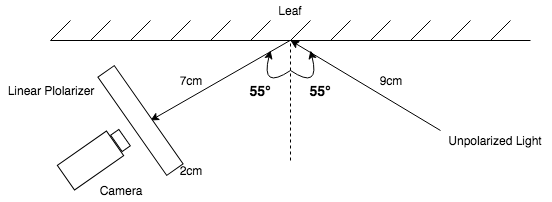
\includegraphics[scale=0.5]{/Sources/Experimental_Design/specular-exp.png}}
    \end{center}
    \caption{Specular Experimental Setup}
    \label{fig:Experiment}
\end{figure}
\begin{figure}[!htb]
    \begin{center}
        \makebox[\textwidth]{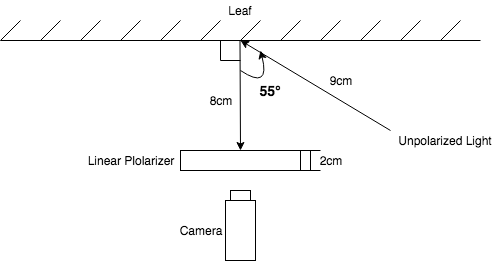
\includegraphics[scale=0.5]{/Sources/Experimental_Design/diffuse-experiment.png}}
    \end{center}
    \caption{Diffuse Experimental Setup}
    \label{fig:Experiment}
\end{figure}
%
Using measurements acquired through a linear polarizer, the polarizance of each sample was calculated and plotted as a histogram.  The measurements were acquired using a digital microscope which produced images for each orientation of the polarizing filter.  These images were additionally processed for texture feature extraction using GLCM techniques.

Each color image was split into its individual color channel to apply greyscale imaging techniques for pseudo-spectral analysis.

Extracted features were observed and utilized for the purpose of classification among species, and determining the relative water content of individual leaves using regression analysis.  For each type of experiment the same orientation of polarizer and camera was used to capture images in the diffuse and specular directions.

  %%%%%%%%%%%%%%%%%%%%%%%%%%%%%%%%%%%%%%%%%%%%
\chapter{Data Acquisition}
%%%%%%%%%%%%%%%%%%%%%%%%%%%%%%%%%%%%%%%%%%%%
\begin{center}
  \begin{minipage}{0.75\textwidth}
    \begin{small}
      “I went to the woods because I wished to live deliberately, to front only the essential facts of life, and see if I could not learn what it had to teach, and not, when I came to die, discover that I had not lived”.\\
      \null\hfill\emph{Walden. Henry David Thoreau}
    \end{small}
  \end{minipage}
  \vspace{0.5cm}
\end{center}

Images were acquired using a digital microscope through various polarization filter arrangements in order to determine each materials polarization and texture properties.  A broadband white light source was utilized to illuminate the target under investigation.  The DOP of the light source was found to be low, 0.02 \text{\%}. The lights within the room were turned off during data acquisition to reduce the amount of ambient light noise.  In real world applications any ambient light should be accounted for using radiometric calibration techniques or other correction methods.  A custom web application was created to capture, label and store images for easy access and processing.  The acquired data and processing code can be found in \cite{noob}.

%%%%%%%%%%%%%%%%%%%%%%%%%%%%%%%%%%%%%%%%%%%
\section{Measurement of Stokes Parameters}
%%%%%%%%%%%%%%%%%%%%%%%%%%%%%%%%%%%%%%%%%%%
The Stokes parameters for a beam of light can be determined by measuring the flux values of orthogonal polarization states.  A variety of optical setups can be required to measure all of the Stokes parameters.  A Classical polarimeter is one that utilizes a rotating quarter wave plate in front of a linear polarizer to sample a sine wave from the intensities recorded by a detector.  A Fourier analysis is then performed on this signal to determine all of the Stokes parameters.

It is shown in \cite{chipman} that the Stokes parameter of a beam can be generally calculated as
%
\begin{align}
    \mathbf{S} =
    \begin{bmatrix}
        S_0 \\
        S_1 \\
        S_2 \\
        S_3
    \end{bmatrix}
    =
    \begin{bmatrix}
        P_H + P_V \\
        P_H - P_V \\
        P_P - P_M \\
        P_R - P_L
    \end{bmatrix}
    \frac{watts}{m^2}
\end{align}
%
where $P_H, P_V, P_P, P_M, P_R$ and $P_L$ represent flux measurements recorded through filters that extinguish orthogonal polarization states. This is a discrete polarimetric measurement and calculation.

For most natural and man made objects, the reflections are assumed to contain little or no circular polarization. The last row of the Stokes vector is therefore left out of the discussion and the equation becomes
%
\begin{align}
    \mathbf{S} =
    \begin{bmatrix}
        S_0 \\
        S_1 \\
        S_2
    \end{bmatrix}
    =
    S_0
    \begin{bmatrix}
        P_H + P_V \\
        P_H - P_V \\
        P_P - P_M
    \end{bmatrix}
\end{align}
%
The linear elements of the Stokes vector can be determined using just a linear polarizer and rotating the polarizer to 0, 45, 90 and 135 degrees.  These measurements are denoted $P_H, P_P, P_V$ and $P_M$. They represent the captured time average intensities for the $S$ and $P$ components of the electric field previously described in section $2.1.4$.
%
%ßß\begin{center}
%  \makebox[\textwidth]{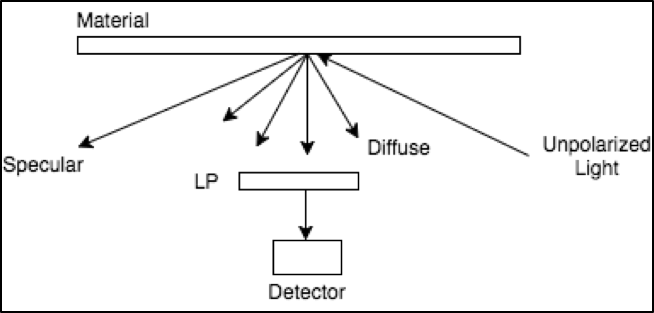
\includegraphics[width=8cm]{Sources/Background/Data_Acquisition/exper_setup.png}}
%\end{center}
%
The linear polarizer was calibrated using a polarizer of known axis orientation.  The calibration polarizer was kept with its axis constant to the S plane of the material.  The lens of the measurement polarizer was rotated until a null intensity was reached and the axis of transmission for the polarizer was orthogonal to that of the calibration polarizer.  The polarizer has a known extinction ratio of 19 and a polarization of \text{95\%} efficiency.  The spectral response across the visible spectrum is shown in Figure 4.1.  It shows that the polarizer produces a constant response across the visible range of the energy spectrum.

\begin{figure}[!htb]
    \begin{center}
        \makebox[\textwidth]{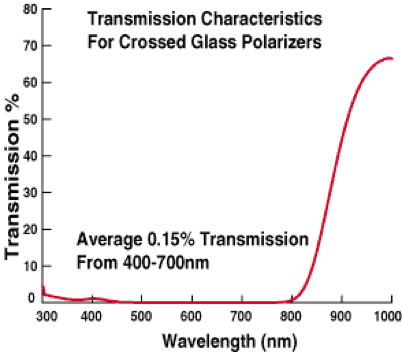
\includegraphics[scale=0.75]{/Sources/Data_Acquisition/polarizer-charac.png}}
    \end{center}
    \caption{Polarizer Characteristic from Edmund Optics}
    \label{fig:polarization}
\end{figure}
When unpolarized light is incident, the Stokes vector for the exiting beam is identical to the polarizance of the Mueller matrix for the material and can be useful for classification of materials.  This reduction in form was shown in Equation 2.64.

The intensity measurement is recorded with a USB powered, digital microscope acting as a detector.

%%%%%%%%%%%%%%%%%%%%%%%%%%%%%%%%%%%%%%%%%%%
\section{Single and Multi-Pixel Detectors}
%%%%%%%%%%%%%%%%%%%%%%%%%%%%%%%%%%%%%%%%%%%
For centuries the only photo detector available to those in the field of optics was the human eye.  Many methods were only capable of producing measurements via a null intensity method, where light was extinguished to determine orthogonality between polarization and polarizer transmission axes.  Modern single pixel photo detectors allow for the capturing of intensity or tone.  There are numerous types of detectors available which are made from materials that exhibit different properties when interacting with light.  Silicon is a common substrate.

A single pixel is not enough to capture texture.  Multiple measurements need to be made using a single pixel in order to quantify a region of space around the surface, denoted by the units of steradians in the BRDF models.  Multi-pixel detectors with a larger field of view allow for multiple features and texture to be captured in an image.

A camera is made up of a pattern of multiple silicon photodetectors and filters.  The most common filter arrangement is that of a Bayer filter.  This pattern consists of red, green, and blue spectral filters arranged as shown in Figure 4.2.
\begin{figure}[!htb]
    \begin{center}
        \makebox[\textwidth]{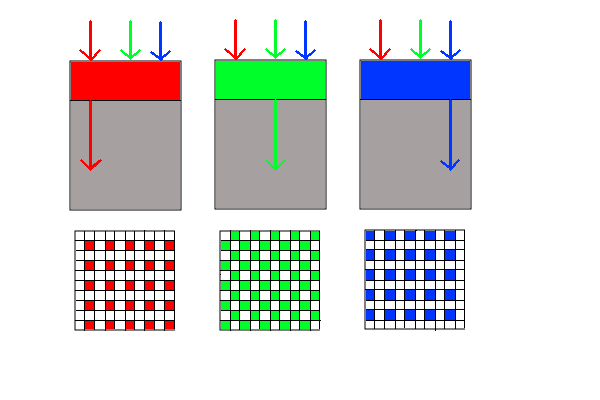
\includegraphics[scale=0.5]{/Sources/Data_Acquisition/bayerfilter-v2.png}}
    \end{center}
    \caption{Bayer Filter Pattern}
    \label{fig:polarization}
\end{figure}
%
The individual intensities from each of these filters are captured by the camera and used to create a three-channel RGB representation of the image scene.  Each channel represents the intensity of a given pixel for the color filter in the Bayer pattern.

Single and multi-pixel devices have been utilized in Polarimetry for different applications.  In these experiments a digital microscope was used as it provides information on texture as well as an ability to distinguish features in each of the spectral color channels.

The intensity values for each RGB channel of an image can easily be extracted using the OpenCV Python package.  Note that OpenCV actually holds images in reverse order as BGR.

OpenCV, a popular image processing library in Python, stores images as intensities in a multidimensional array representing the blue, green, and red response patterns.  It is possible to separate these channels and access the discrete intensity values to perform a pseudo-spectral analysis.

%%%%%%%%%%%%%%%%%%%%%%%%%%%%%%%%%%%%%%%%%%%
\section{Determining Relative Water Content}
%%%%%%%%%%%%%%%%%%%%%%%%%%%%%%%%%%%%%%%%%%%
The steps for determining the RWC involve weighing the leaf in its current water state, artificially hydrating the leaf to its maximum capacity and completely drying out the leaf.  The procedure for obtaining the measurements necessary for obtaining the RWC are as follows \cite{ecophysiology},\cite{rwc:1},

1.	Remove leaf from host plant leaving approximately 2 cm of petiole

2.	Weigh leaf to acquire the Fresh Leaf Weight (FW)

3.	Place leaf petiole in solution of distilled water and ${CaCl}_2$ at 2mM for at least 8 hours

4.	Weigh leaf to acquire Turgid Weight (TW)

5.	Place leaf in an oven at 60 \textdegree C for 4 days

6.	Weigh leaf to acquire the Dry Weight (DW)


The relative water content can then be calculated as a percentage,
%
\begin{align}
    RWC = \frac{FW - DW}{TW - DW} x 100%
\end{align}
%
Note that the scale used for weighing needs to have at least 4 decimal places to ensure the accuracy of the measurements. Drying times and artificial hydration times can vary with species and oven temperature. An example of measurements can be found in Table 4.1.  All acquired RWC data can be found in the Appendix.
%
\begin{table}[htb]
  \centering
  \begin{tabular}{lllll}
    \toprule
    \textbf{Leaf} & \textbf{TFW (g)} & \textbf{TW (g)} & \textbf{DW(g)} & \textbf{RWC \%} \\
    \midrule
      \texttt{11} & 2.7931 & 2.8335 & 0.2472 & 98.4379 \\
      \texttt{12} & 2.0883 & 2.1184 & 0.1876 & 98.4411 \\
      \texttt{21} & 1.7804 & 1.8051 & 0.1376 & 98.5187 \\
      \texttt{22} & 1.7655 & 1.8022 & 0.1404 & 97.7916 \\
      \texttt{31} & 2.1874 & 2.2359 & 0.1656 & 97.6573 \\
      \texttt{32} & 2.2511 & 2.3108 & 0.1687 & 97.2130 \\
      %
      \texttt{1\_1} & 1.3687 & 1.3807 & 0.0826 & 99.0756 \\
      \texttt{1\_2} & 1.6860 & 1.7015 & 0.1024 & 99.0307 \\
      \texttt{2\_1} & 1.4904 & 1.4904 & 0.1029 & 97.0378 \\
      \texttt{2\_2} & 2.2324 & 2.2690 & 0.2003 & 98.2308 \\
      \texttt{3\_1} & 1.2877 & 1.3003 & 0.1070 & 98.9441 \\
      \texttt{3\_2} & 1.7654 & 1.7825 & 0.1330 & 98.9633 \\
      %
      \texttt{1+1} & 2.1297 & 2.1586 & 0.1667 & 98.5491 \\
      \texttt{1+2} & 1.5341 & 1.5699 & 0.0973 & 97.5689 \\
      \texttt{2+1} & 1.1938 & 1.3323 & 0.0867 & 88.8809 \\
      \texttt{2+2} & 2.2729 & 2.4420 & 0.2165 & 92.4017 \\
      \texttt{3+1} & 1.5755 & 1.6441 & 0.1314 & 95.4651 \\
      \texttt{3+2} & 2.3954 & 2.4486 & 0.2114 & 97.6220 \\
      %
      \texttt{3\&1} & 1.6107 & 1.6478 & 0.1380 & 98.4379 \\
      \texttt{3\&2} & 2.3541 & 2.4297 & 0.1987 & 98.4411 \\
      \texttt{3\&3} & 1.6821 & 1.7432 & 0.1758 & 98.5187 \\
      \texttt{3\&4} & 2.0762 & 2.1322 & 0.2168 & 97.7916 \\
      \texttt{3\&5} & 1.1001 & 1.1153 & 0.0823 & 97.6573 \\
      \texttt{3\&6} & 2.0207 & 2.2154 & 0.1737 & 97.2130 \\
      %
      \texttt{1.1} & 1.1294 & 1.1478 & 0.0702 & 98.2925 \\
      \texttt{1.2} & 1.0425 & 1.0525 & 0.0631 & 98.9893 \\
      \texttt{2.1} & 1.2669 & 1.2905 & 0.0987 & 98.0198 \\
      \texttt{2.2} & 1.0833 & 1.0961 & 0.0769 & 98.7441 \\
      \texttt{3.1} & 1.0311 & 1.0377 & 0.0872 & 99.3056 \\
      \texttt{3.2} & 1.2738 & 1.2820 & 0.1097 & 99.3005 \\
      %
      \texttt{3\textasciicircum1} & 1.1240 & 1.1462 & 0.0959 & 97.8863 \\
      \texttt{3\textasciicircum2} & 1.5232 & 1.5917 & 0.1597 & 95.2165 \\
      \texttt{3\textasciicircum3} & 1.4585 & 1.4826 & 0.1218 & 98.2290 \\
      \texttt{3\textasciicircum4} & 1.0184 & 1.0504 & 0.0822 & 96.6949 \\
      \texttt{3\textasciicircum5} & 1.3605 & 1.3605 & 0.0967 & 97.6974 \\
      \texttt{3\textasciicircum6} & 1.2660 & 1.2660 & 0.0935 & 97.9446 \\
      %
    \bottomrule
  \end{tabular}
  \caption{%
    Measurements for RWC Experiment using Equation 4.3
  }
  \label{tab:Packages}
\end{table}
%

  %%%%%%%%%%%%%%%%%%%%%%%%%%%%%%%%%%%%%%%%%%%%
\chapter{Feature Extraction}
%%%%%%%%%%%%%%%%%%%%%%%%%%%%%%%%%%%%%%%%%%%%
\begin{center}
  \begin{minipage}{0.75\textwidth}
    \begin{small}
      “Movement amongst the trees of a forest shows that the enemy is advancing.  The appearance of a number of screens in the midst of this grass means that the enemy wants to make us suspicious”.\\
      \null\hfill\emph{The Art of War, Sun Tzu}
    \end{small}
  \end{minipage}
  \vspace{0.5cm}
\end{center}

After acquiring the necessary images for calculation of a leafs' polarizance, features were extracted from the images in each color channel for texture and polarization analysis.  These features were extracted using various Python programming modules. One hundred samples were extracted from each image to randomly create a training and testing set of data.  Diffuse and specular datasets were processed separately.

In order to create testing and training data, samples were extracted from each polarization image $H, V, P$ and $M$ using code found in Figure 5.1.  Each sample was extracted into three different color channels; red, green and blue.

\begin{figure}
    \begin{lstlisting}
        def extract_bgr_samples(filename, size, count):
            """
            Extract random samples from b, g, r image channels.

            Args:
                filename (str): Location to the image filename.
                size (int): The length/width of the square sample.
                count (int): The number of samples to generate.
            Returns:
                tuple: Random samples from each color channel.
            """
            img = cv2.imread(filename, 75, 1)
            samples = image.extract_patches_2d(img, (size, size), count, 1)
            cv2.imwrite('sample.png', samples[0])
            b, g, r = bgr_split(samples[0])

            return b, g, r
    \end{lstlisting}
    \caption{Extract samples from each BGR Image Channel Example Code}
    \label{fig:scattering}
\end{figure}

This type of function mentioned in Figure 5.1 can be used to extract sample patches from all three (BGR) color channels. Features can then be extracted from each of the color samples.  An example grey level histogram and image for each individual color channel through an H polarization filter can be found in Figures 5.2, 5.3 and 5.4.
\begin{figure}
    \begin{center}
        \makebox[\textwidth]{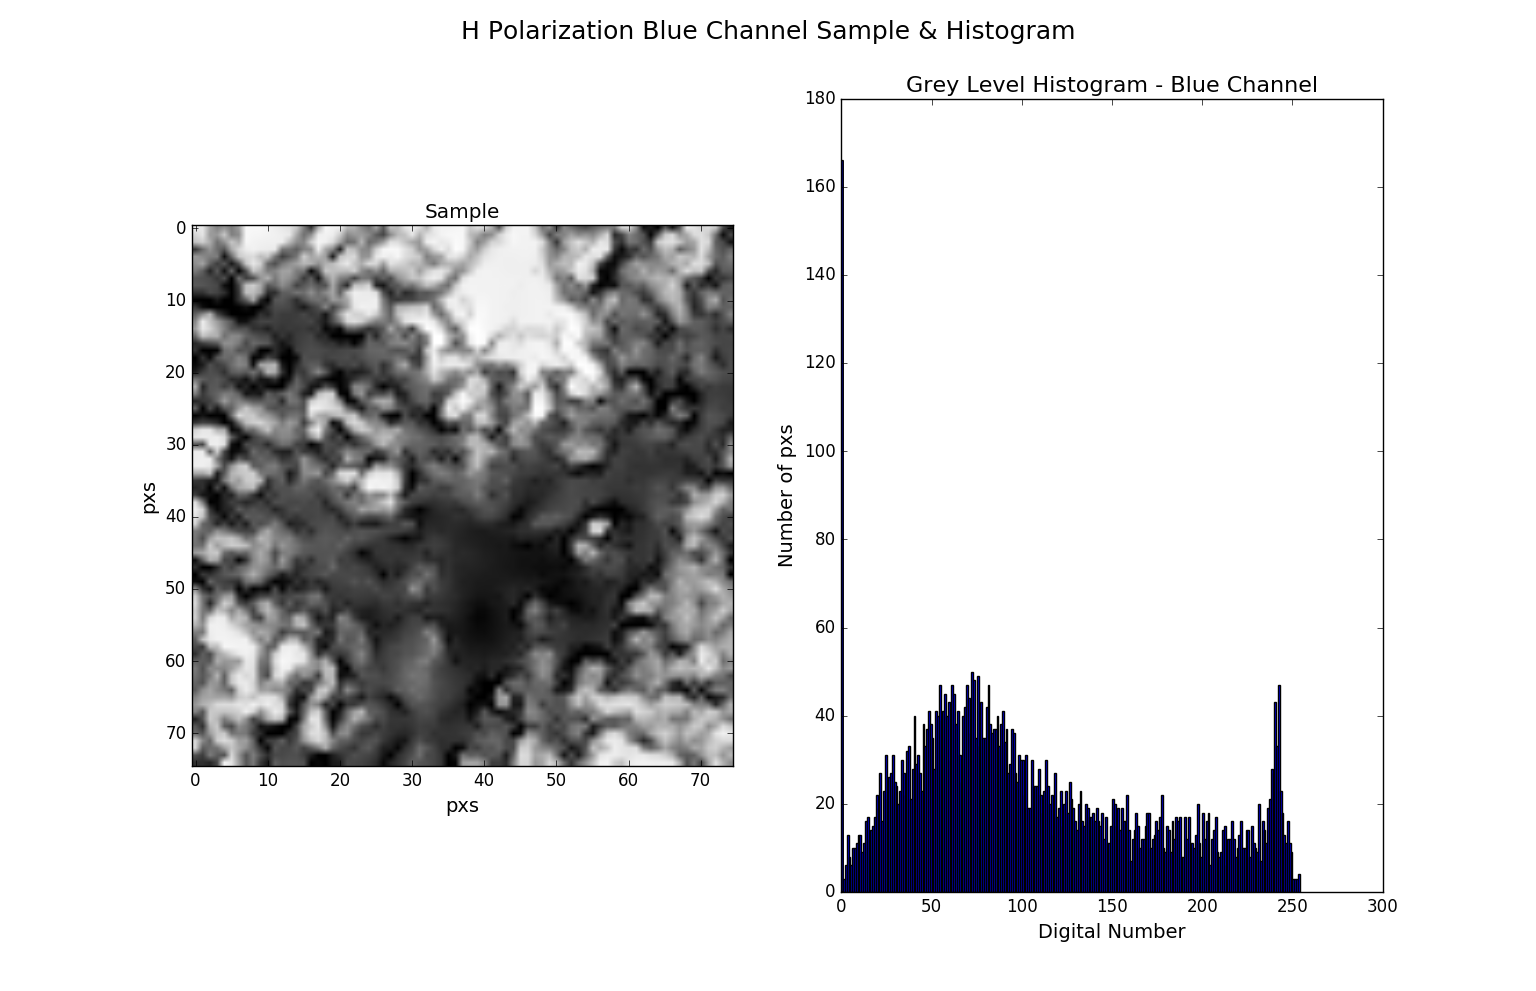
\includegraphics[scale=0.35]{/Sources/Feature_Extraction/di-H-blue-sample-hist.png}}
    \end{center}
    \caption{Devils Ivy Blue Channel H Filter Histogram}
    \label{fig:polarization}
\end{figure}
\begin{figure}
    \begin{center}
        \makebox[\textwidth]{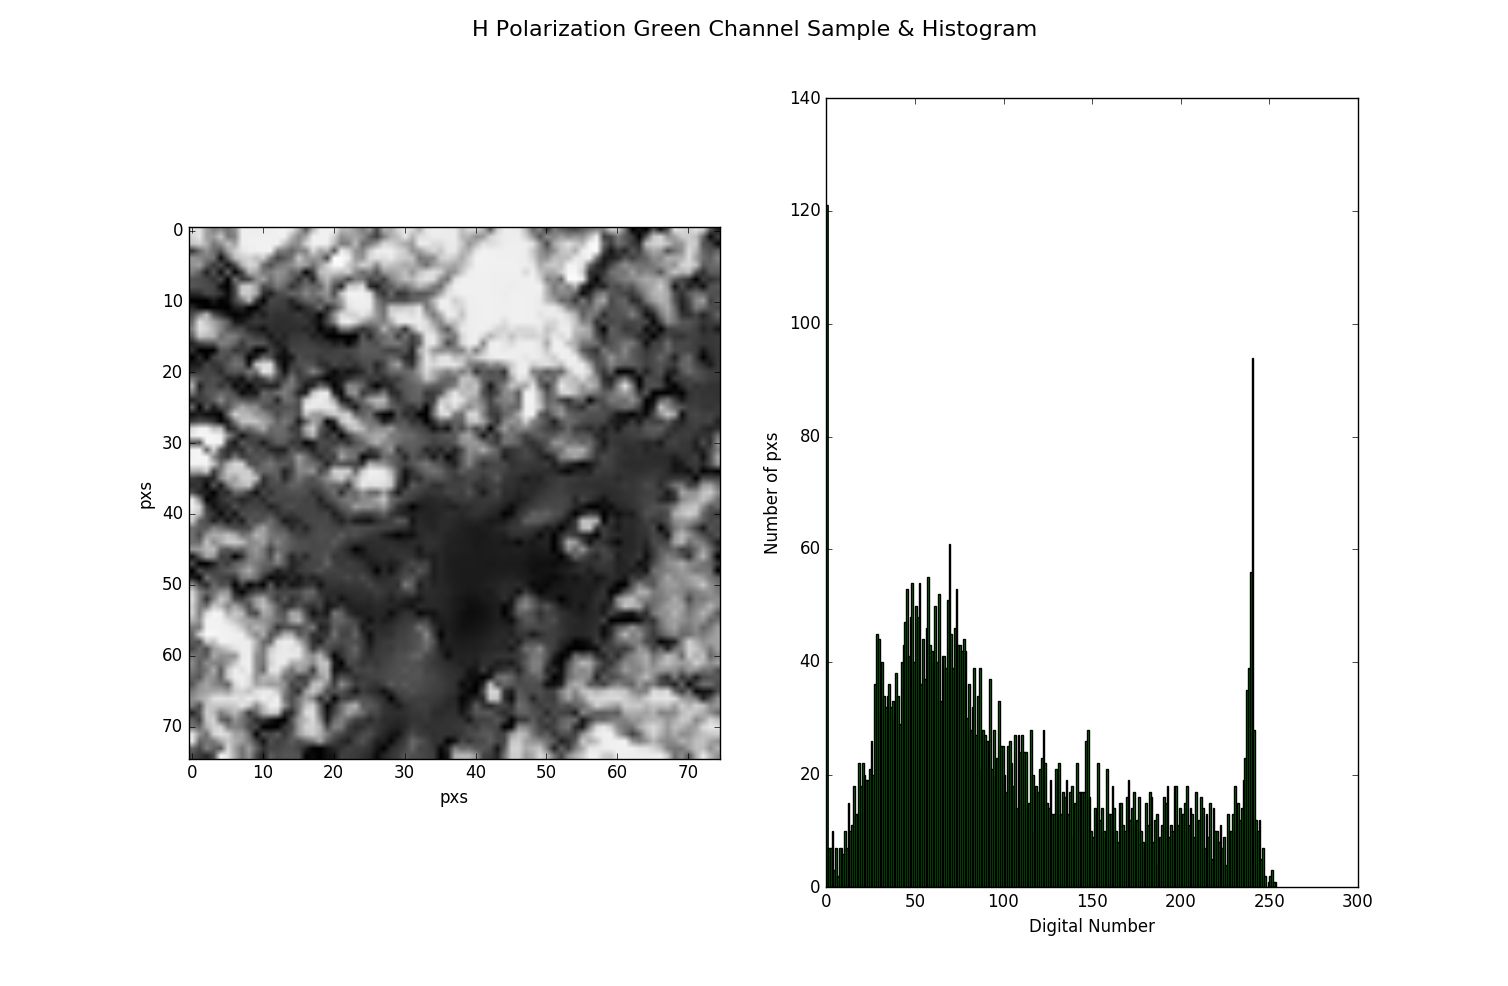
\includegraphics[scale=0.35]{/Sources/Feature_Extraction/di-H-green-sample-hist.png}}
    \end{center}
    \caption{Devils Ivy Green Channel H Filter Histogram}
    \label{fig:polarization}
\end{figure}
\begin{figure}
    \begin{center}
        \makebox[\textwidth]{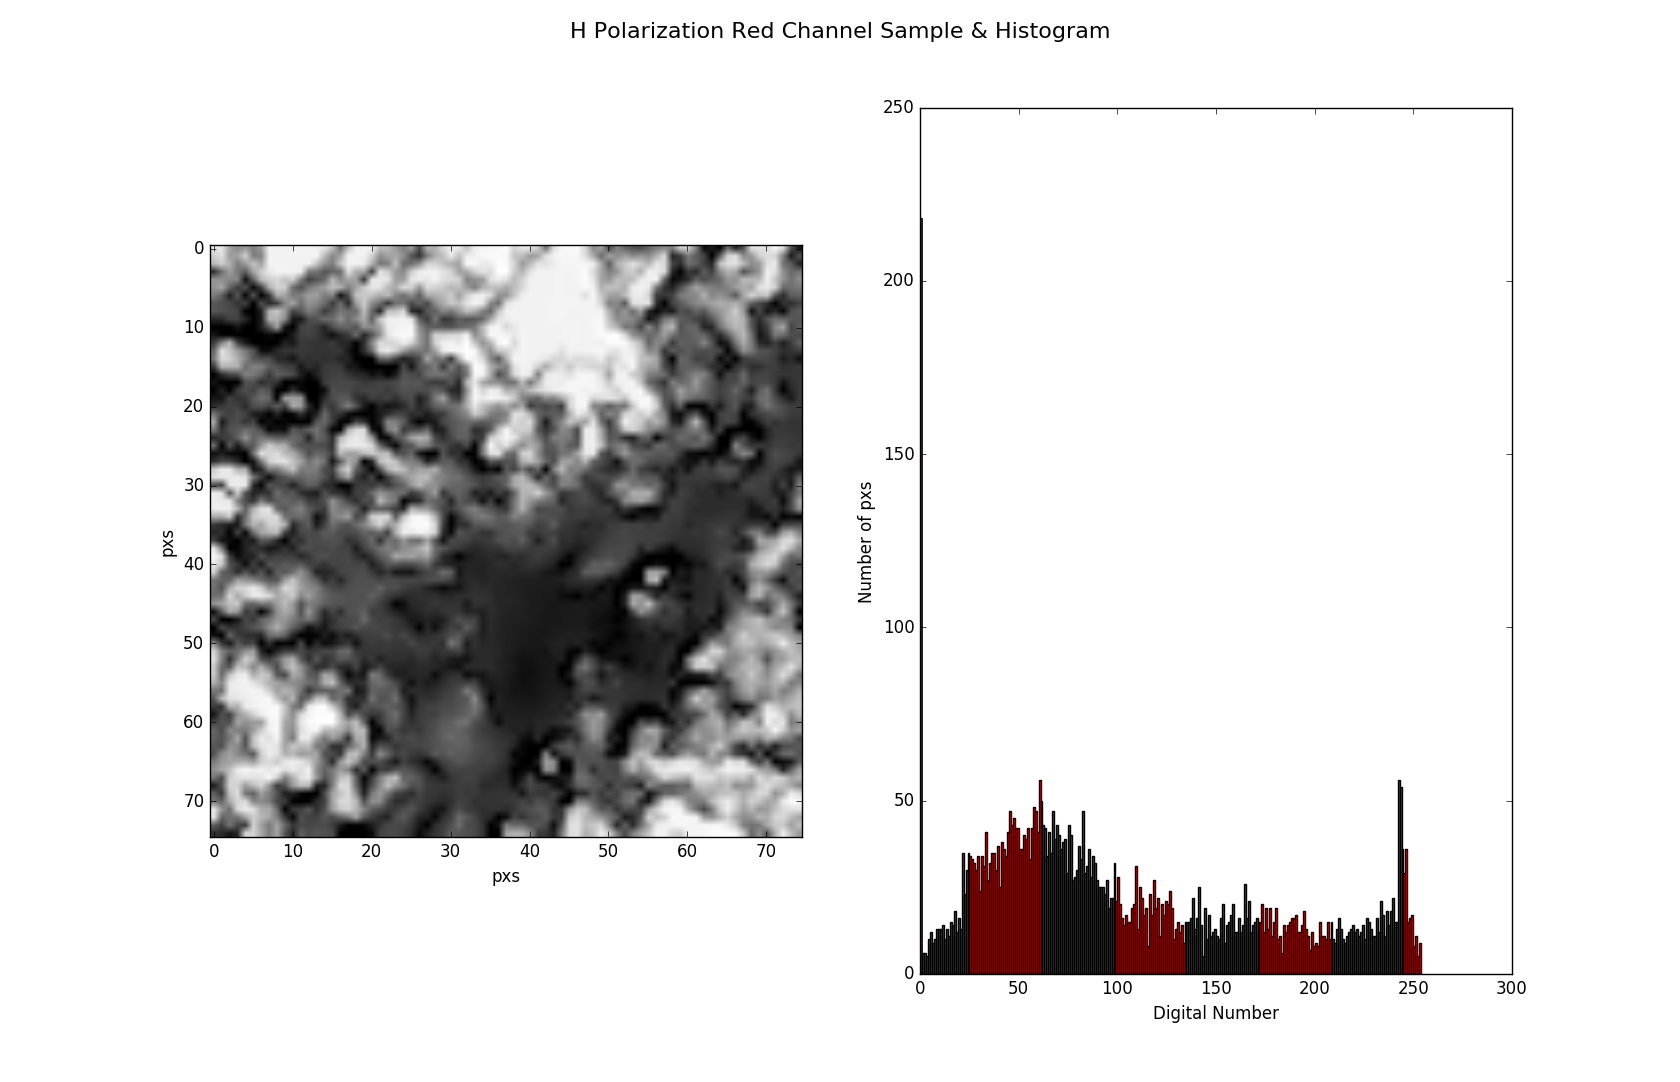
\includegraphics[scale=0.33]{/Sources/Feature_Extraction/di-H-red-sample-hist.png}}
    \end{center}
    \caption{Devils Ivy Red Channel H Filter Histogram}
    \label{fig:polarization}
\end{figure}
The corresponding V filter channels are found in Figures 5.5, 5.6 and 5.7 for a 75x75 pixel sample of Devils Ivy.
\begin{figure}
    \begin{center}
        \makebox[\textwidth]{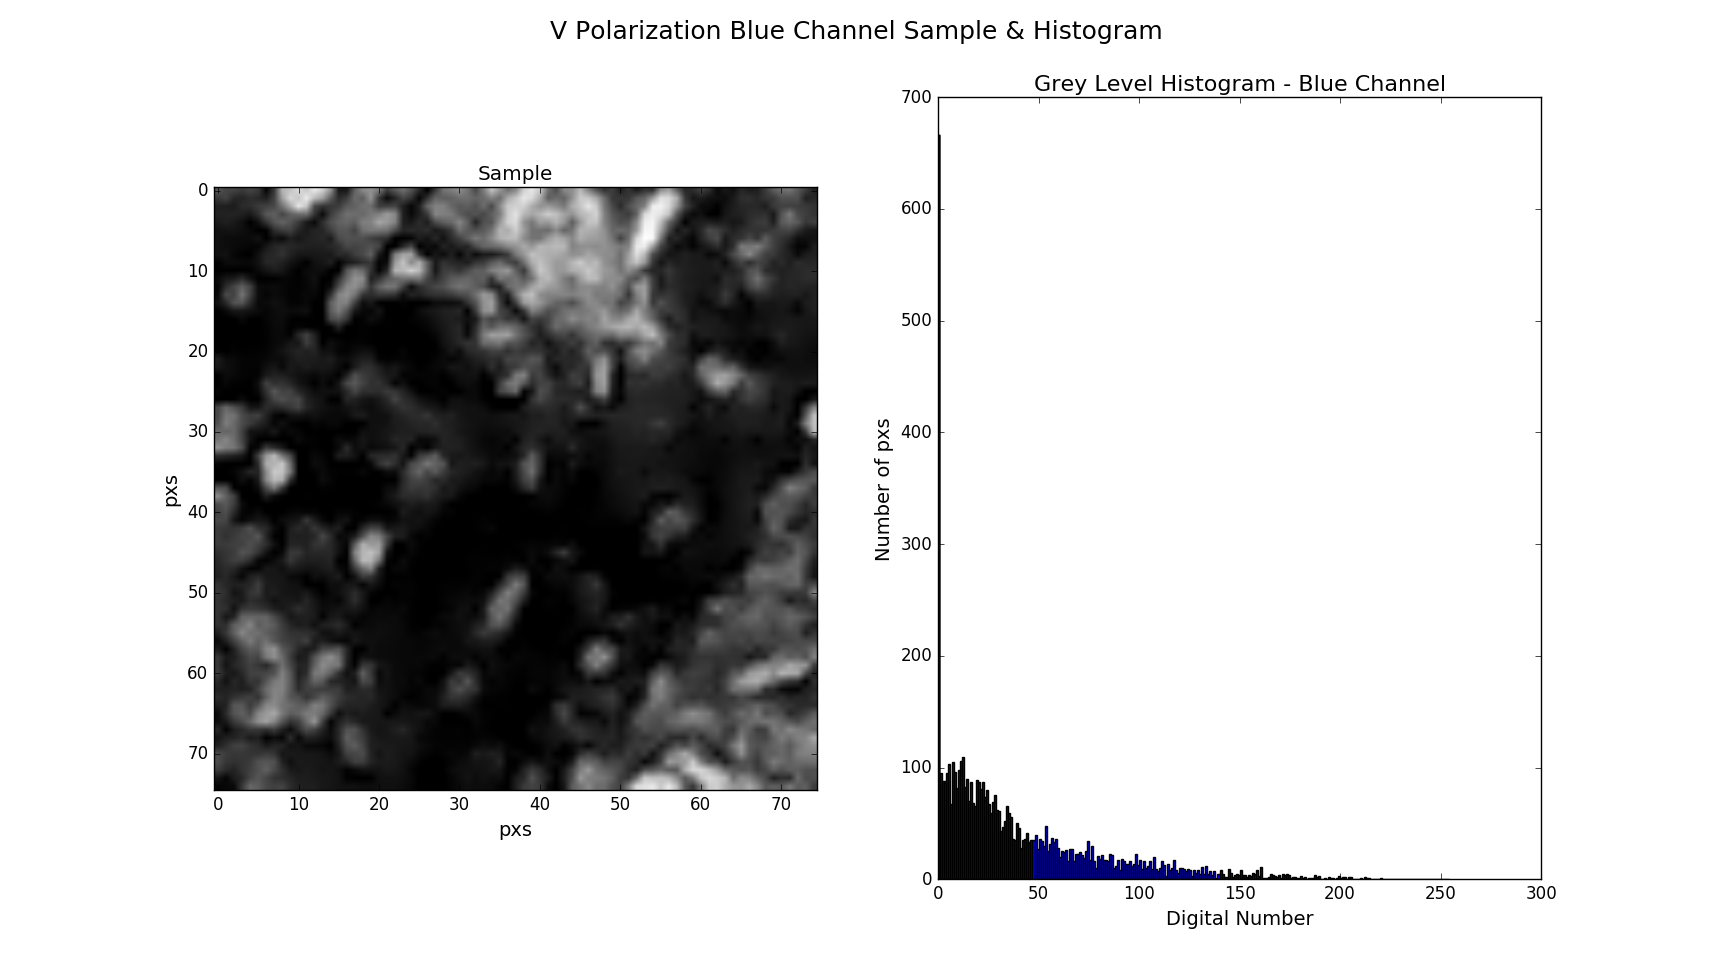
\includegraphics[scale=0.35]{/Sources/Feature_Extraction/di-V-blue-sample-hist.png}}
    \end{center}
    \caption{Devils Ivy Blue Channel V Filter Histogram}
    \label{fig:polarization}
\end{figure}
\begin{figure}
    \begin{center}
        \makebox[\textwidth]{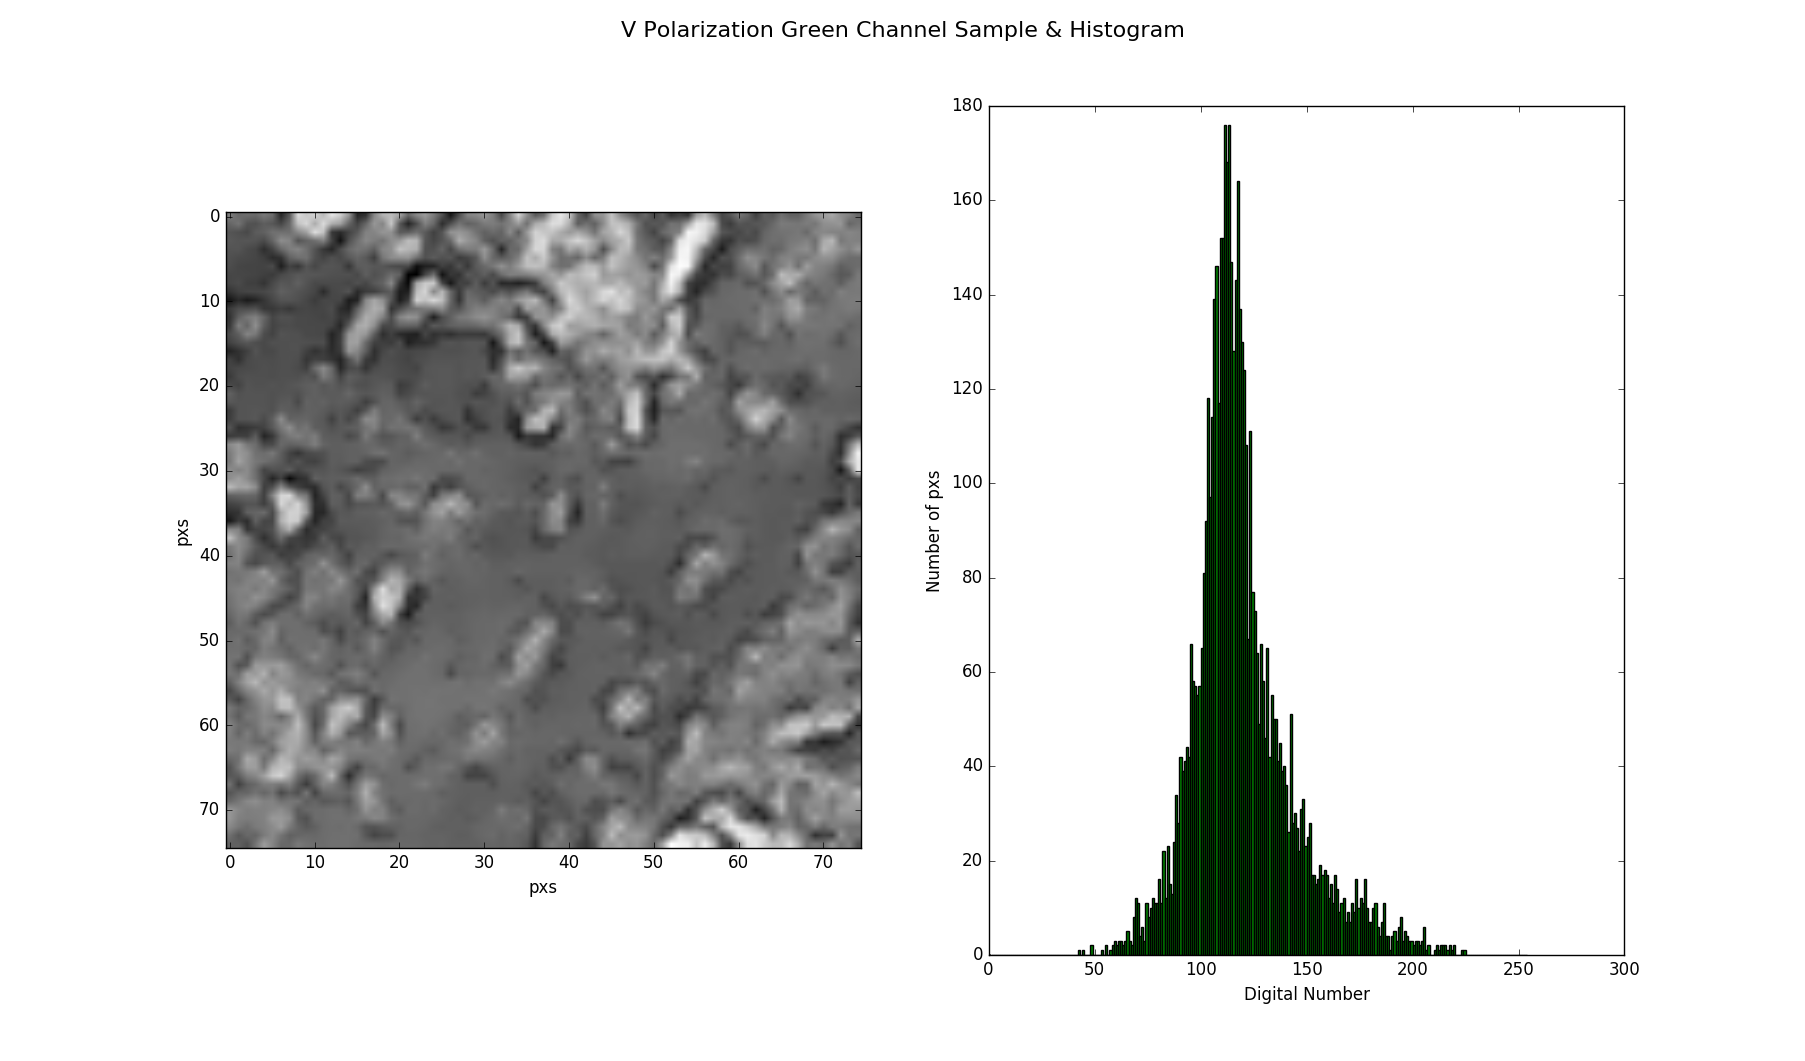
\includegraphics[scale=0.35]{/Sources/Feature_Extraction/di-V-green-sample-hist.png}}
    \end{center}
    \caption{Devils Ivy Green Channel V Filter Histogram}
    \label{fig:polarization}
\end{figure}
\begin{figure}
    \begin{center}
        \makebox[\textwidth]{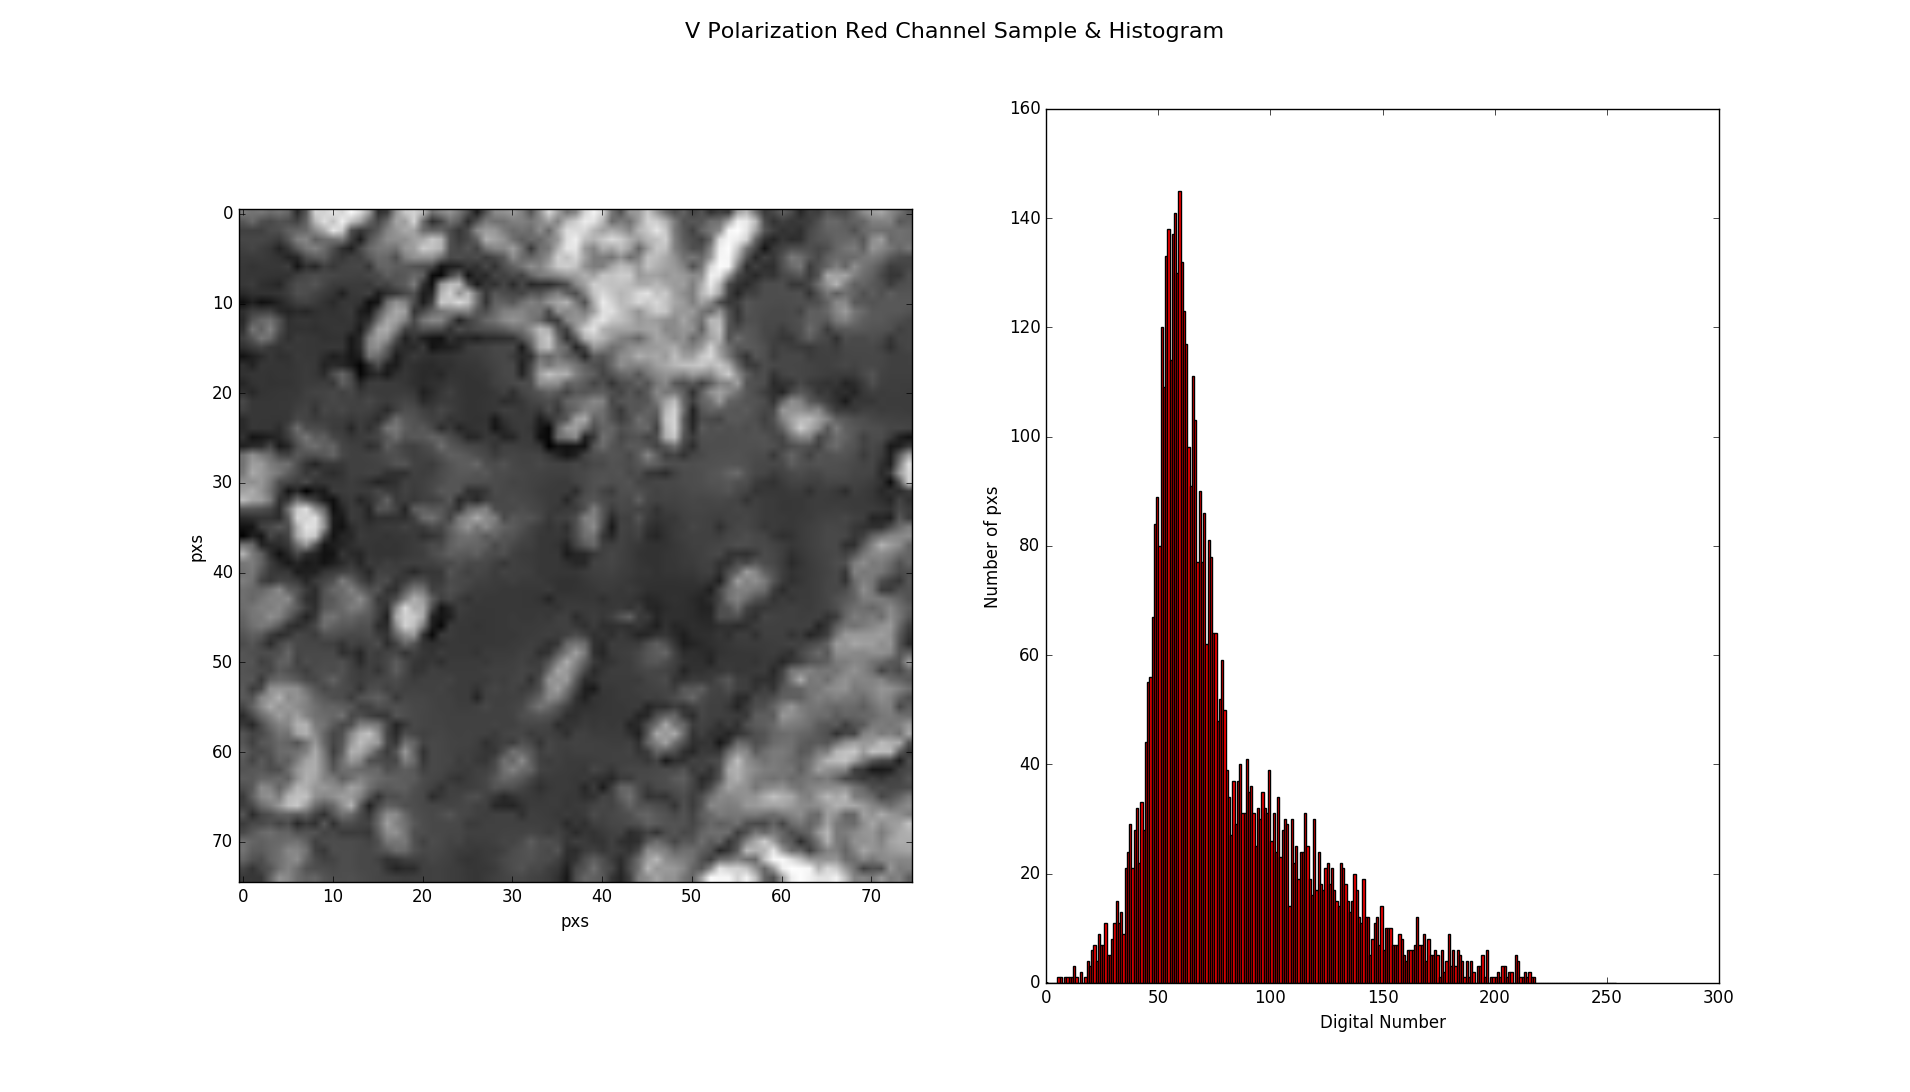
\includegraphics[scale=0.31]{/Sources/Feature_Extraction/di-V-red-sample-hist.png}}
    \end{center}
    \caption{Devils Ivy Red Channel V Filter Histogram}
    \label{fig:polarization}
\end{figure}
Each of the samples were processed using pixel based analysis, to calculate their Stokes vector as well as various GLCM metrics.  Pixels that were never illuminated were filtered out of the polarization analysis since they artificially inflated the zero mean of the produced histograms.  Polarization is not the same as light intensity and polarization cannot be determined without some illumination on the target.  The Stokes vector was calculated using the code in Figure 5.8 where P1 and P2 represent orthogonal flux measurements through a linear polarizer.
%
\begin{figure}
    \begin{lstlisting}
        def calculate_stokes((P1, P2)):
            """
            Calulate the Stokes parameter for orthogonal images.

            Args:
                P1 (array): First polarization image.
                P2 (array): Orthogonal polarization image.
            Returns:
                array: Stokes parameters.
            """
            P1 = P1.astype(np.float32)
            P2 = P2.astype(np.float32)

            P1[np.abs(P1) < 1] = 0
            P2[np.abs(P2) < 1] = 0

            S = (P1 - P2) / (P1 + P2)

            # These represent values that have not been illuminated by the source
            # ie they are the product of masking and shadowing.
            S[~np.isfinite(S)] = 0

            return S
    \end{lstlisting}
    \caption{Example Code for Calculating the Stokes Parameters}
    \label{fig:scattering}
\end{figure}
%
These values were binned into histograms in order to reduce the dimensionality and storage requirements for the data.  These histograms were plotted using the following code in Figure 5.9.
%
\begin{figure}
    \begin{lstlisting}
        S1 = calculate_stokes((H, V))
        S2 = calculate_stokes((P, M))

        plt.title('Polarizance Paramaters')

        plt.hist(S1.ravel(), histtype='barstacked', bins=256)
        plt.hist(S2.ravel(), histtype='barstacked', bins=256)

        plt.show()
    \end{lstlisting}
    \caption{Calculate and Plot the Stokes Parameters}
    \label{fig:scattering}
\end{figure}
%
The resulting polarization histograms for a Devils Ivy sample can be found in Figure 5.10 for each corresponding BGR channel.  A false image has also been included which shows the absolute value of the S1 polarization for each channel and location on the original image.  The result of creating a false image out of the a polarization matrix, allows for a visualization for how polarization is resulting from specific surface and subsurface features.
\begin{figure}
    \begin{center}
        \makebox[\textwidth]{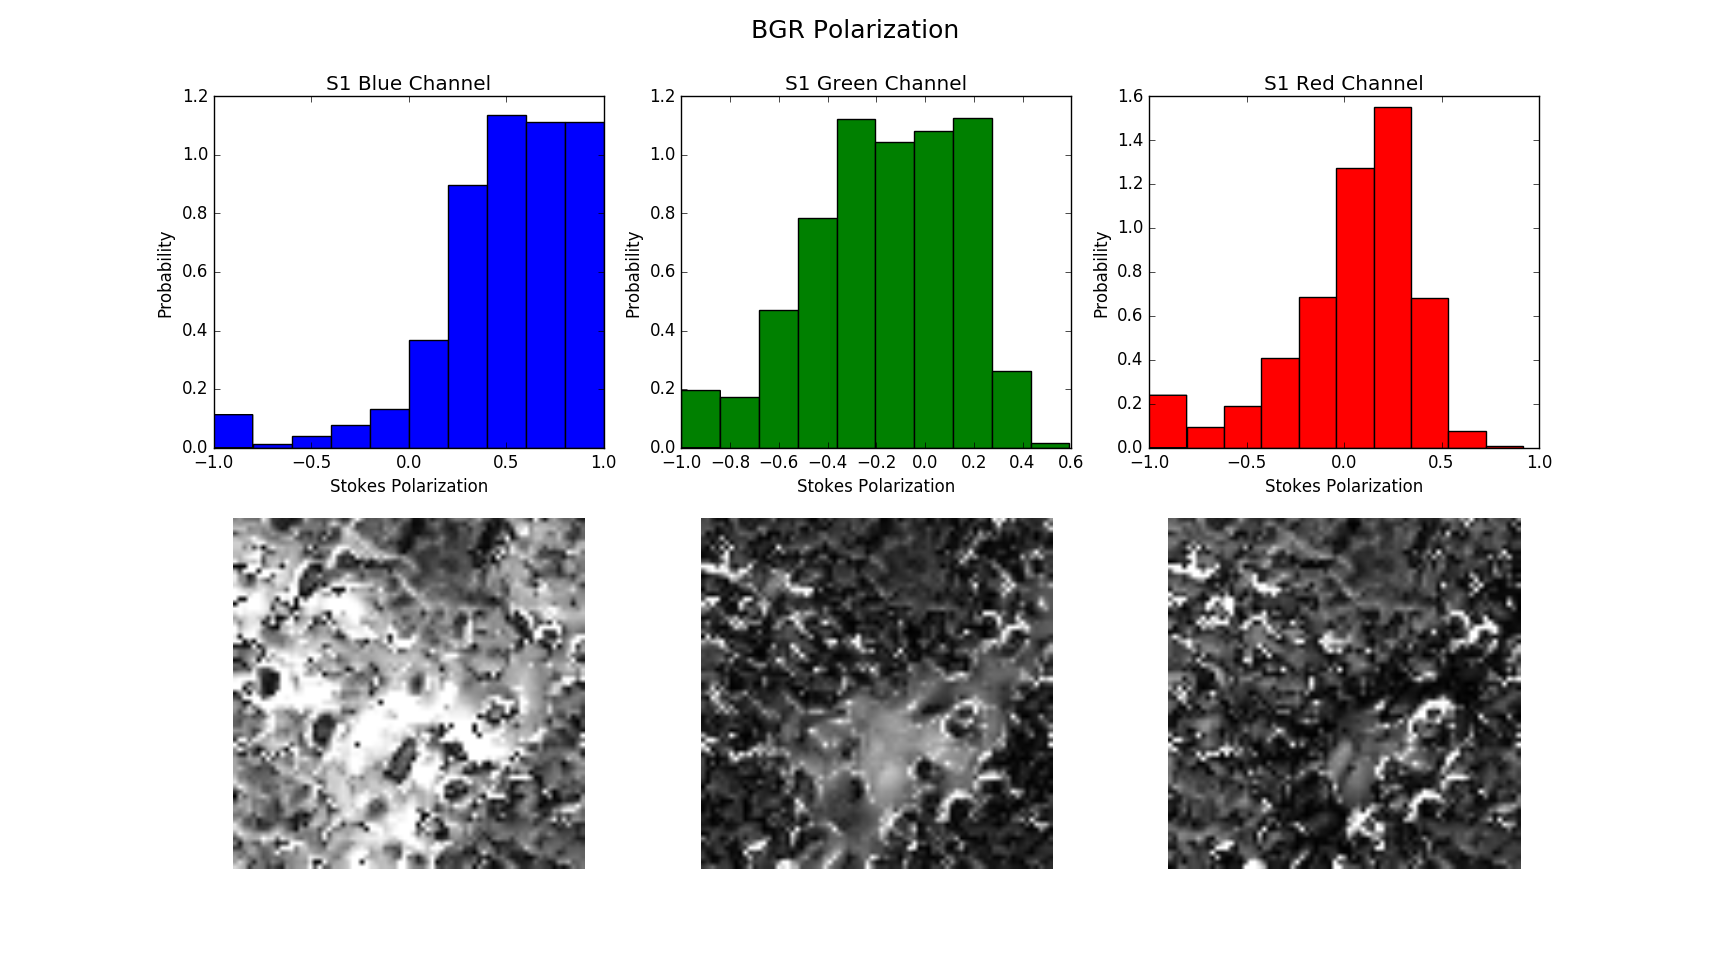
\includegraphics[scale=0.35]{/Sources/Feature_Extraction/di-bgr-s1-v2.png}}
    \end{center}
    \caption{BGR Histograms for Devils Ivy Sample S1 Polarization Parameter}
    \label{fig:polarization}
\end{figure}
Window-based GLCM texture analysis was similarly performed on each of the extracted samples.  The dissimilarity, correlation, contrast and entropy were calculated for each GLCM.  The window size for GLCM was manually optimized by testing clustering effects for 5px, 9px, 25px, 55px, 75px, and 95px window sizes.  A window size of 75 pixels was found to be ideal for this experimental design.

In addition to performing a polarization based analysis on each color channel of the extracted samples, a GLCM texture analysis was also performed.  The dissimilarity, contrast, correlation and energy were calculated for each sample window.  The code in Figure 5.11 was used for these calculations,
\begin{figure}
    \begin{lstlisting}
        def extract_texture(samples):
            """
            Generate GLCM based texture features for a given color channel.

            Args:
                samples (array): Array containing each image sample.  Each sample is a
                    matrix of pixel intensities for a single color channel.
            Returns:
                array: Texture features extracted for an individual color channel.
            """
            texture = []
            for sample in samples:
                try:
                    # Calculate texture features for a given sample
                    relationships = [0, np.pi/4, np.pi/2, 3*np.pi/4]
                    glcm = greycomatrix(sample, [1], relationships, 256, symmetric=True, normed=True)
                    metrics = ['dissimilarity', 'contrast', 'correlation', 'energy']
                    diss, contrast, corr, energy = [greycoprops(glcm, metric)[0, 0] for metric in metrics]

                    texture.append([diss, contrast, corr, energy])
                except ValueError:
                    print "Error in extracting the texture features"

            return np.array(texture)
    \end{lstlisting}
    \caption{Code to Extract GLCM Features From Texture Samples}
    \label{fig:scattering}
\end{figure}
The metrics derived from the GLCM matrix can be plotted in various scatterplots as demonstrated in the Results chapter and Appendix. Data was exported to .csv files for future processing and analysis in Support Vector Machine classification and linear regression.
Pixel-based, histogram counts and GLCM derived, window-based metrics were combined to form feature vector sets in the classification and regressions given in Chapter 7.

  %%%%%%%%%%%%%%%%%%%%%%%%%%%%%%%%%%%%%%%%%%%%
\chapter{Classification and Regression Analysis}
%%%%%%%%%%%%%%%%%%%%%%%%%%%%%%%%%%%%%%%%%%%%
\begin{center}
  \begin{minipage}{0.75\textwidth}
    \begin{small}
      “The interaction between material bodies can be described either by formuating the action at a distance between the interacting bodies or by separating the interaction process into the production of a field by one system and the action so the field on another system” .
      \emph{Classical Electricity \& Magnetism. Panofksy, Phillips}\\.
    \end{small}
  \end{minipage}
  \vspace{0.5cm}
\end{center}

\section{Support Vector Machines}
A Support Vector Machine (SVM) is binary classification tool that is used in machine learning classification and regression problems.  SVMs attempt to separate data by creating a hyper plane that maximizes the distance between each of the classes.  This is often performed in high dimensional spaces, where each sample is described by multiple features.

The python package Sci-Kit Learn provides access to SVM modules and utilities that make it easy to run analysis on datasets.  This packages allows for easily performing machine learning classification and cross validation.  Pipelines are setup for streamlining any preprocessing steps before classification.  This allows for easy modification and testing of various steps in the machine learning process.  A pipeline can be setup in order to allow for easy access to the classifier processing steps during analysis such as,
%
\begin{lstlisting}
from sklearn import svm
from sklearn.multiclass import OneVsRestClassifier
from sklearn.preprocessing import StandardScaler

clf = OneVsRestClassifier(make_pipeline(
	StandardScaler(),
	svm.SVC(kernel='linear', probability=True)))

\end{lstlisting}
%
The OneVsRestClassifier was used to extend binary classification methods to multiclass problems, allowing for the use of SVC to classify Red Oak, American Ash and Sugar Maple leaves.  The chosen kernel was linear.  The GridSearch module of sklearn can additionally be utilized to find the most optimal parameters for fitting the data, when free parameters are available.

In Support vector classification, the C and epsilon are tunable parameters.

\subsection{Validation of Classifier Results}
Cross validation of results is important for reducing the training and testing bias inherent to some datasets.  Learning curves are useful visualization tools for showing how adding more samples to a testing set effects the classification score or ability.

A stratified K-fold validation can be used for ensuring that when sets of training and testing sets are created, the testing sets contain equal amounts of each class.  This is especially useful in unequally distributed sets of data.

In binary classification problems, it is of interest to understand the ability of a classifier to correctly predict the true condition of the sample under inspection.  The possible outcomes of a classification can be found in Figure
% TODO create ROC boxes
A true positive result is one that correctly identifies the sample.  False negatives incorrectly predict that a sample was not in its own class.  False positives are when samples are incorrectly identified with another class.  True negatives correctly identify that a sample is not a member of the class being tested against.   These rates can be combined into useful metrics for quantifying a classifiers performance.

The precision of a classifier is a measure of the relevancy of its results.  It is an overall indicator of the false positive rate of a classifier.
%
\begin{align}
    P = \frac{T_p}{T_p + F_p}
\end{align}
%
were $T_p$ is the number of true positives and $F_p$ is the number of false positives that result from testing on the trained classifier.  The recall, also known as the sensitivity, is defined as
%
\begin{align}
    R = \frac{T_p}{T_p + F_p}
\end{align}
%
and tells the amount of relevant samples returned and $F_n$ is the false negative rate.  The f1 score is the harmonic mean between the precision and recall, and is defined as,
%
\begin{align}
    F1 = 2\frac{PR}{P + R}
\end{align}
%
The classification report shows a useful cross validated summary of the precision, recall, f1 score, and support vectors that results from testing different dataset.

All of these features are available in the Sklearn package and an example is shown below.
%
\begin{lstlisting}
from sklearn.model_selection import classification_report, StratifiedKFold

cv = StratifiedKFold(2, shuffle=True)

for train, test in cv.split(X, y):
    y_test = label_binarize(y[test], classes=[0,1,2, 3])

    fit = clf.fit(X[train], y[train])

    y_pred = fit.predict(X[test])

    print classification_report(y[test], y_pred)
\end{lstlisting}
%
These metrics are often visualized using receiver operating characteristic (ROC) curves for binary classification, and confusion matrices for multiclass problems.  ROC curves show the sensitivity vs the specificity of a binary classifier by plotting the false positive rate versus the true positive rate.  It “is a graphical plot that illustrates the diagnostic ability of a binary classifier system as its discrimination threshold is varied” [wiki]. The area under the ROC curve, often denoted AUC, is a measure equivalent to the score of a classifier. It should be noted that for multiclass problems ROC curves can be more optimistic than the individual performance metrics.

ROCs can be extended to multiclass problems, by using a one verse many techniques although a confusion matrix is often used to show the accuracy of a classifier between each of the various classes.  A confusion matrix shows the classifier score against each combination of true value and predicted value.  It therefore shows all outcomes of classification.

It is important to understand the bias and variance of a model when determining its overall effectiveness.  The bias is the average error for different training sets while the variance indicates how sensitive a model is to varying training sets.

Learning curves are a useful visualization tool for understanding the bias and variance of a classification model.  It is useful for determining if a model gets better at classifying samples, as the number of training samples increases.  If the score of a classifier decreases as the number of samples increases, the model has a high amount of bias.  The model performs is not generalized enough to handle more training data.  If as the number of training samples increases, the score increases, the model could benefit from more training data.  If the score remains constant as the training samples increase, the model has low bias.

\section{Linear Regression}

  %%%%%%%%%%%%%%%%%%%%%%%%%%%%%%%%%%%%%%%%%%%%
\chapter{Results}
%
\begin{center}
  \begin{minipage}{0.75\textwidth}
    \begin{small}
      “I hear and I forget. I see and I remember. I do and I understand”\\
      \null\hfill\emph{Confucius}
    \end{small}
  \end{minipage}
  \vspace{0.5cm}
\end{center}
\section{Optimization of Parameters}
The histograms that resulted from measuring the S1 and S2 polarization showed evidence of masking and shadowing effects due to macro level surface features.  This caused some pixels to never be illuminated and have a large spike at zero.

Pixels that were never illuminated were removed from the histogram process. These were determined by checking if PH, PV, PP, and PM never had a value more than 0.  This removed the spike at zero.

The free parameters in Support Vector Classification were optimized using the Sklearn grid search module.

%%%%%%%%%%%%%%%%%%%%%%%%%%%%%%%%%%%%%%%%%%%%%
\section{Classification}
%%%%%%%%%%%%%%%%%%%%%%%%%%%%%%%%%%%%%%%%%%%%%
Images were acquired for each polarization filter orientation. Red Oak, American Ash, and Sugar Maple leaves were measured immediately after being removed from their host tree and polarization measurements were recorded.  The same procedure was then performed 1 week later.  These measurements produce interclass variance and show the effects of the decomposition process on the polarization response and texture of various leaf species.  In total 18 different leaves were investigated for classification purposes under experimental design setup 1.  Images were acquired in both the specular and diffuse directions for each leaf.  100 samples of 75 by 75 pixels were extracted from each leaf to represent various textures found on the surface and the physiological status below the surface.  In total 1800 samples were used to perform classification and validation using a linear support vector classifier.
%%%%%%%%%%%%%%%%%%%%%%%%%%%%%%%%%%%%%%%%%%%%%%
\subsection{Specular Leaves}
%%%%%%%%%%%%%%%%%%%%%%%%%%%%%%%%%%%%%%%%%%%%%%
%
\begin{figure}[htp]
    \centering
    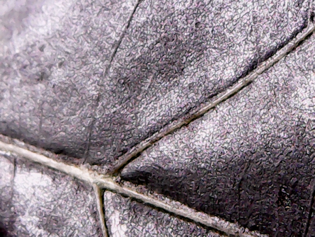
\includegraphics[width=.3\textwidth]{/Sources/Results/721/oak-raw.png}\hfill
    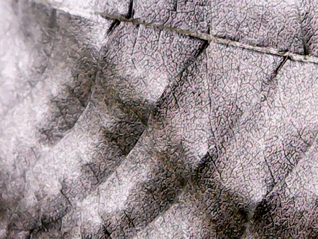
\includegraphics[width=.3\textwidth]{/Sources/Results/721/Ash-raw.png}\hfill
    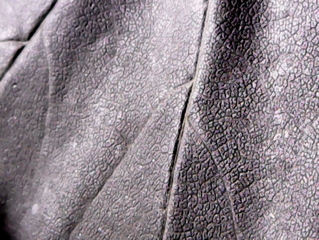
\includegraphics[width=.3\textwidth]{/Sources/Results/721/sugar-raw.png}

    \caption{From left to right: Red Oak, American Ash, and Sugar Maple through H polarization filter in the Specular Direction.}
    \label{fig:specular-raw}
\end{figure}
%
The principles of reflection and transmission as dictated by Fresnel’s equations show that light reflecting from a specular surface will have higher amounts of polarization than when compared with the diffuse direction.  The S1 component for all leaves showed this response as expected and produced higher amounts of polarization than when compared to their diffuse counterparts.  The S2 component showed itself to have a near zero mean, with some variance.

The histograms for the S1 and S2 parameters comparing different tree leaves were computed for the blue, green and red camera channels.  These individual channels in general are the same as the overall grey level image shown as RGB here, although more distinguished features can be seen in Figure 19 for each individual channel.
%
\begin{figure}[!htb]
    \begin{center}
        \makebox[\textwidth]{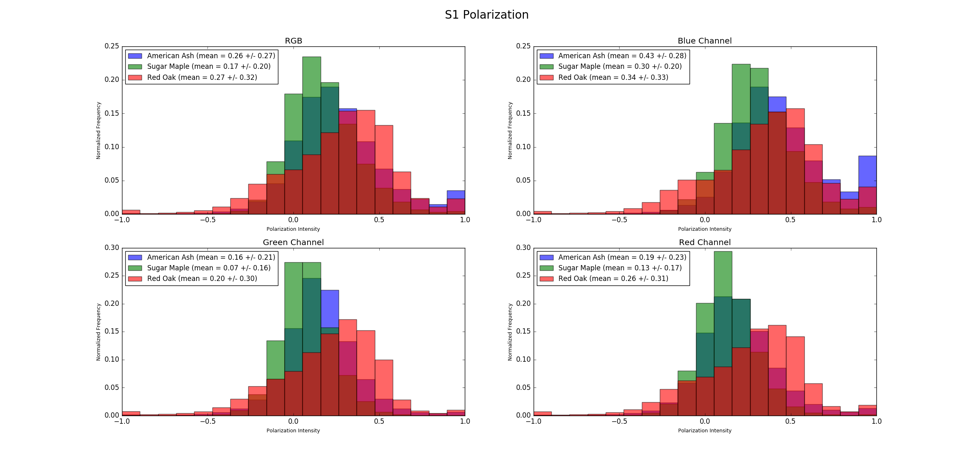
\includegraphics[scale=0.9]{/Sources/Results/721/allhistpolarization.png}}
    \end{center}
    \caption{All plants specular observed direction for each RGB channelization 0 week for S1}
    \label{fig:polarization}
\end{figure}
%
The blue and red channel show higher amounts of polarization, while the green channel shows the least amount of polarization, across each species.  It has previously been shown, that Rayleigh scattering on a leafs' surface can greatly increase the polarization in the blue spectrum of light [26].  Since plants reflect highly in the green, the green channel shows the lowest amount of polarization.  The blue channel shows the most amount of polarization, although this may be due to the sensitivity of the CMOS sensor as shown in Figure 14 or Rayleigh scattering [26].  The blue channel is extended to regions of red light and therefore is overall more sensitive in the visible region to spectral fluctuations.  Perhaps in the future, the blue channel response should be subtracted from the red channel response, and the blue channel can be normalized using the following ratio,
%
\begin{align}
    Blue_{calibration} = Blue - (Blue - Red)
\end{align}
%
Ideally the response of each channel would be carefully calculated using a spectrometer, and overall constants could be provided to normalize the sensitivity in each spectral region.  This requires various narrow band spectral filters.

The S2 histograms in Figure 20 show very little polarization on average.  This is expected polarization angles at 45 and 135 can be decomposed into X and Y components.  It is possible that the S2 component could be useful in understanding the calibration of the linear polarizer to its ideal orientation.  If P and M measurements diverge drastically, it would serve as a notion to investigate the variance further for specular reflections.
%
\begin{figure}[!htb]
    \begin{center}
        \makebox[\textwidth]{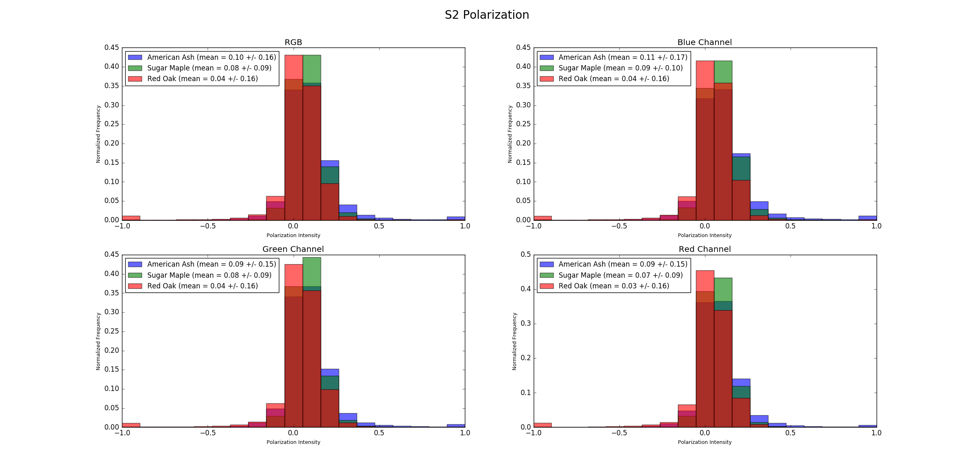
\includegraphics[scale=0.9]{/Sources/Results/721/all-s2-polarization.png}}
    \end{center}
    \caption{All plants RGB channels observed from the specular direction 0 week for S2}
    \label{fig:polarization}
\end{figure}
%
The specular direction of observation and incident angle at the Brewster angle creates the highest amount of polarized light on an ideal smooth surface.  Leaves can also be seen to similarly have specular components that correlate to the surface topology.

A GLCM texture analysis was also performed on each sample extracted to determine the dissimilarity, contrast, entropy, and correlation. Due to each of the GLCM features being generated from the same initial matrix, many of the features show high levels of correlation.  In general, a measure should be taken from the orderliness group, contrast group and descriptive statistics group. It has previously been shown [mayer source] that a textures dissimilarity and correlation show low levels of correlation.  Therefore, they are plotted here to represent the texture in 2 dimensions.

Although these features contain information regarding the texture of a surface, it is often difficult to determine what actually causes each metric to arise when describing specific surface GLCM properties [4].

Figure 21 shows the texture of the leaves above for the V filter orientation.  It shows that each species exhibits its own unique texture that helps to visually create clusters, and therefore should prove useful for classification.
%
\begin{figure}[!htb]
    \begin{center}
        \makebox[\textwidth]{\includegraphics[scale=0.9]{/Sources/Results/721/all_glcm.png}}
    \end{center}
    \caption{V filter GLCM dissimilarity and correlation for all species in the specular direction week 0}
    \label{fig:polarization}
\end{figure}
%
Additional filter arrangements can be found in the Appendix.

\subsection{Specular Leaf Decomposition}
As leaves start to undergo pigment breakdown and decomposition, the surfaces of the leaves provide more reflectance.  The loss of water and pigment structure results in rougher external surface on the leaf that causes a more diffuse reflection, even when viewed at the Brewster angle.  This results in a loss of magnitude of S1 polarization as the leaf decomposes.  Visual changes to the surface of the leaf can be found in the original V filter images.
%
\begin{figure}[htp]
    \centering
    \hspace*{\fill}%
    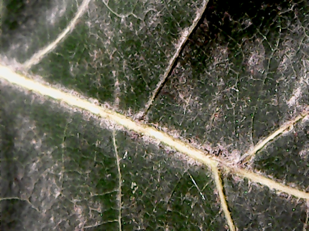
\includegraphics[width=.3\textwidth]{/Sources/Results/7_2_2/oak_new_raw.png}\hfill%
    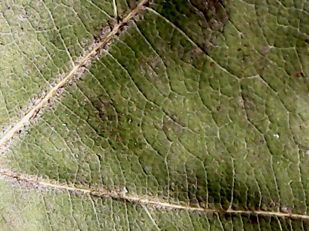
\includegraphics[width=.3\textwidth]{/Sources/Results/7_2_2/Oak_raw_1wk.png}
    \hspace*{\fill}%
    \caption{From left to right: Red Oak Freshly Removed and After One Week}
    \label{fig:specular-raw-decompose}
\end{figure}
%
Close inspection Figure 22 and Figure 21 show that the new leaf is a darker green in color and has a smoother surface than the oak leaf after 1 week.  The smooth, thick wax surface as it ages from week 0 to week 1, becomes flatter and segmentation of structures on the leaf surface becomes more evident.

Recording the leaves after one week to illustrate changes during decomposition and water loss for red oak can be seen in Figure 24.  It should be noted that the blue channel contains a large amount of polarization after one week. In some cases, it has been seen to even exceed its 0-week counterpart. This may be due to the absorbance spectrum of chlorophyll and the lack of photosynthetic activity during decomposition. The overall S1 image shows the 0 week has higher polarization in S1 as its surface is more of a pure specular reflector.
%
\begin{figure}[!htb]
    \begin{center}
        \makebox[\textwidth]{\includegraphics[scale=0.9]{/Sources/Results/7_2_2/s1_polar.png}}
    \end{center}
    \caption{Red Oak 0 weeks and 1 week observed in the specular direction for S1}
    \label{fig:polarization}
\end{figure}
%
\begin{figure}[!htb]
    \begin{center}
        \makebox[\textwidth]{\includegraphics[scale=0.9]{/Sources/Results/7_2_2/s2_polar.png}}
    \end{center}
    \caption{Red oak 0 weeks and 1 week observed in the specular direction for S2}
    \label{fig:polarization}
\end{figure}
%
Again S2 only shows a slight variation even after re-measuring the leaf one week later.

The results of GLCM analysis for the P filter component can be found in Figure 26.  Visual inspection of the GLCM scatter plot shows the best clustering using the P filter for this particular example.  The full GLCM filter set can be found in the Appendix.
%
\begin{figure}[!htb]
    \begin{center}
        \makebox[\textwidth]{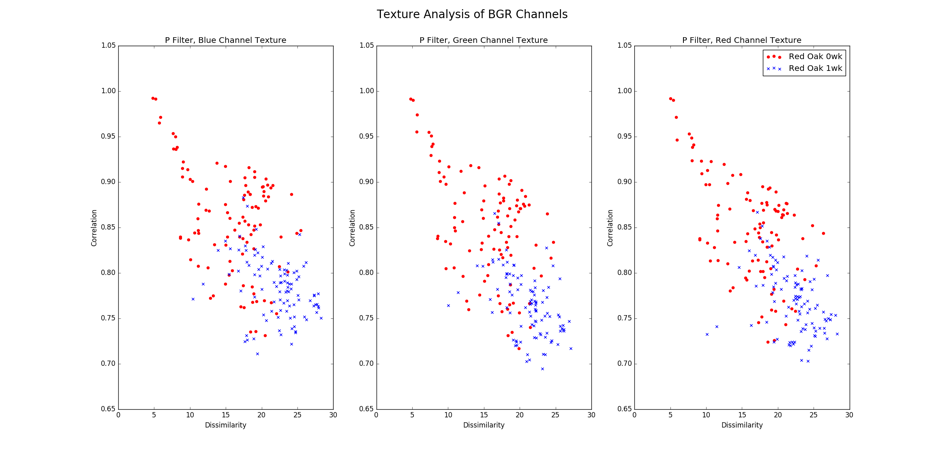
\includegraphics[scale=0.9]{/Sources/Results/7_2_2/glcm_age_specular.png}}
    \end{center}
    \caption{P filter GLCM dissimilarity and correlation in specular direction for 0 and 1 week.}
    \label{fig:polarization}
\end{figure}
%
As water leaves the leaf which undergoes the decomposition process, the surface becomes rougher as the water that once supported much of the cells structure has been removed. The surface becomes more diffuse.  The highly specular component of healthy leaves, creates maximum intensity levels on the cameras detector, making the surface appear smooth.  This results in a higher amount of dissimilarity on the surface of the leaf after one week, as compared to one that is still healthy.  The correlation is shown to also decrease as a result of this process as well.

\subsection{Specular Classification Results}
Classification was performed on datasets created by combining texture samples from leaves that were both zero week and one week old.  This created variance within the classes themselves, as previously it has been shown how physiological changes within the leaf can lead to different polarization and texture results.  The results of classification show that there is still an ability to distinguish between species with a high amount of precision.

The confusion matrix also shows the high level of accuracy when using ten fold stratified K fold validation.  It can be seen that the highest accuracy of classification is when American ash is considered versus Maple or Oak.  Visual inspection of each type of leaf shows the similarity between Oak and Maple when viewed under a microscope, so this result is not unexpected.

A learning curve was also generated for the results of using both texture and polarization features and is shown in Figure 28.  As the number of training samples increases, the score of the classifier remains the same.  This shows the low amount of training bias within the model created from our samples. Future samples should be collected and compared to further validate these results.
%
\begin{figure}[!htb]
    \begin{center}
        \makebox[\textwidth]{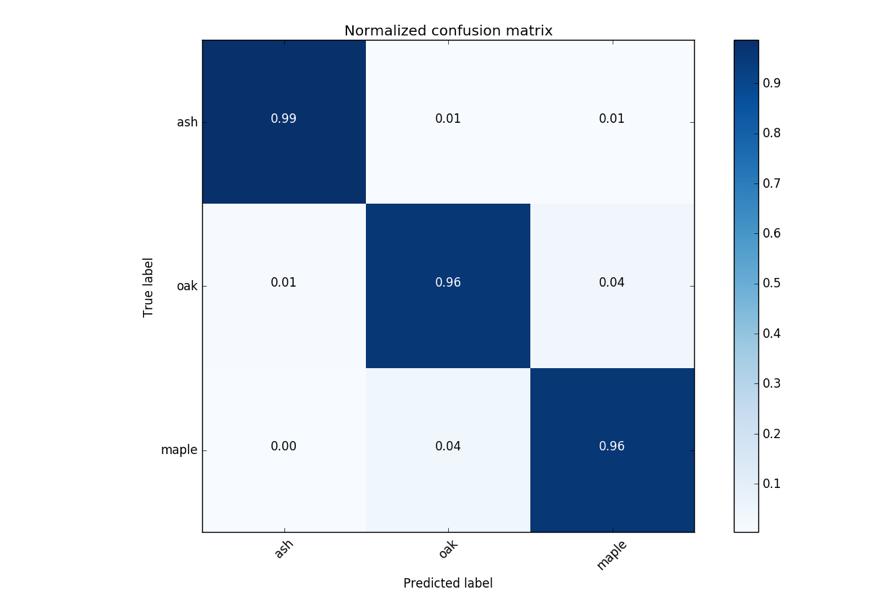
\includegraphics[scale=0.9]{/Sources/Results/7_2_3/confusion.png}}
    \end{center}
    \caption{Confusion Matrix for All Species observed in the specular direction.}
    \label{fig:polarization}
\end{figure}
%
%
\begin{figure}[!htb]
    \begin{center}
        \makebox[\textwidth]{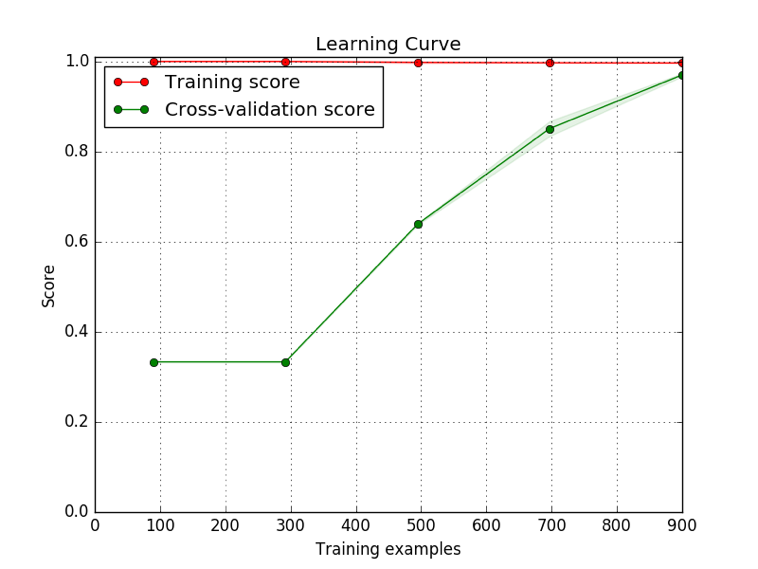
\includegraphics[scale=0.9]{/Sources/Results/7_2_3/learning_curve.png}}
    \end{center}
    \caption{Learning curve for leaves observed in the specular direction.}
    \label{fig:polarization}
\end{figure}
%
The overall results for specular classification for all species using polarization and texture features where class 0 is American Ash, class 1 is Red Oak, and class 2 is Sugar Maple.
%
\begin{table}[htb]
  \centering
  \begin{tabular}{lllll}
    \toprule
    \textbf{Class} & \textbf{Precision} & \textbf{Recall} & \textbf{F1 Score} & \textbf{Support} \\
    \midrule
      \texttt{0.0} & 0.99 & 0.98 & 0.99 & 600 \\
      \texttt{1.0} & 0.95 & 0.95 & 0.95 & 600 \\
      \texttt{2.0} & 0.96 & 0.96 & 0.96 & 600 \\
      \texttt{avg/total} & 0.97 & 0.97 & 0.97 & 1800 \\
    \bottomrule
  \end{tabular}
  \caption{%
    Scores for Classification in the Specular Direction with Polarization and Texture in Specular Direction.
  }
  \label{tab:Packages}
\end{table}
\begin{table}[htb]
  \centering
  \begin{tabular}{lllll}
    \toprule
    \textbf{Class} & \textbf{Precision} & \textbf{Recall} & \textbf{F1 Score} & Support\\
    \midrule
      \texttt{0.0} & 0.95 & 0.97 & 0.96 & 600 \\
      \texttt{1.0} & 0.88 & 0.92 & 0.90 & 600 \\
      \texttt{2.0} & 0.93 & 0.87 & 0.90 & 600 \\
      \texttt{avg/total} & 0.92 & 0.92 & 0.92 & 1800 \\
    \bottomrule
  \end{tabular}
  \caption{%
    Scores for Classification in the Specular Direction with Just Polarization in Specular Direction.
  }
  \label{tab:Packages}
\end{table}
%
\begin{table}[htb]
  \centering
  \begin{tabular}{lllll}
    \toprule
    \textbf{Class} & \textbf{Precision} & \textbf{Recall} & \textbf{F1 Score} & Support\\
    \midrule
      \texttt{0.0} & 0.97 & 0.96 & 0.96 & 600 \\
      \texttt{1.0} & 0.86 & 0.89 & 0.87 & 600 \\
      \texttt{2.0} & 0.90 & 0.87 & 0.88 & 600 \\
      \texttt{avg/total} & 0.91 & 0.91 & 0.91 & 1800 \\
    \bottomrule
  \end{tabular}
  \caption{%
    Scores for Classification in the Specular Direction with Just Texture in Specular Direction.
  }
  \label{tab:Packages}
\end{table}
%
It can be seen that combining both polarization and texture features for classification, results in better precision, recall, and F1 scores than if either of the feature sets are used independently.  This shows the benefit of using different types of features for classification.

\subsection{Diffuse Leaves}
%
\begin{figure}[htp]
    \centering
    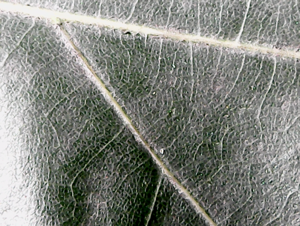
\includegraphics[width=.3\textwidth]{/Sources/Results/7_2_4/oak-raw.png}\hfill
    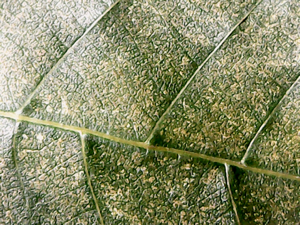
\includegraphics[width=.3\textwidth]{/Sources/Results/7_2_4/ash-raw.png}\hfill
    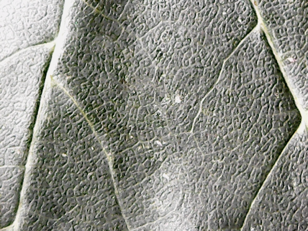
\includegraphics[width=.3\textwidth]{/Sources/Results/7_2_4/maple-raw.png}

    \caption{From left to right: Red Oak, American Ash, and Sugar Maple through H polarization filter in the Diffuse Direction.}
    \label{fig:specular-raw}
\end{figure}
%
Leaves from each species of tree were acquired at 0 degrees from the normal for the plane of incidence.  Examples of each leaf captured through the H filter can be found in Figures 28, 29, and 30.

The diffuse component of reflectance of a leaf is often thought of as being unpolarized.  This assumption if based on a perfect Lambertian diffuse surface, which is often not the case.  Although the portion of polarized light in the diffuse region of reflection is less than that of the specular portion, it cannot be discarded, as it may contain important information as to the biological and physiological processes within the leaf's internal structure.

As photons undergo multiple scattering processes and absorption and reemission by chlorophyll, they can become partially or completely polarized.  These mechanisms are complex, and it is necessary to go beyond Fresnel’s equations to dictate the major processes at work in the diffuse component of scattering.  Polarimetric BRDF models attempt to ascertain the relationship between surface scatter and polarization of light.

Our results show that although the mean is centered around zero for S1, the S2 component shows various degrees of polarization.  These may be due to multiple scattering mechanisms within the layers of the leaf.

The diffuse portion of polarization for each species is shown in Figure 32.
%
\begin{figure}[!htb]
    \begin{center}
        \makebox[\textwidth]{\includegraphics[scale=0.9]{/Sources/Results/7_2_4/s1-polar.png}}
    \end{center}
    \caption{All species, for the diffuse angle of observation 0 week for S1.}
    \label{fig:polarization}
\end{figure}
%
It can be seen that many of the leaves exhibit little to no S1 polarization.  This is expected since much of the S1 polarization results from single scatter surface level phenomena.  The polarization in S2 is shown to be significant.

The polarization can bee seen to be highest in the red and blue where absorption of photons by chlorophyll in the mesophyll layer of the leaf is most prominent.  Structures such as veins may also cause unknown polarization states to result.  Care should be taken when composing images as to what structures are desired for inspection.

The distribution between species in S2 are distributed around different means and variances are as shown in Figure 33.
%
\begin{figure}[!htb]
    \begin{center}
        \makebox[\textwidth]{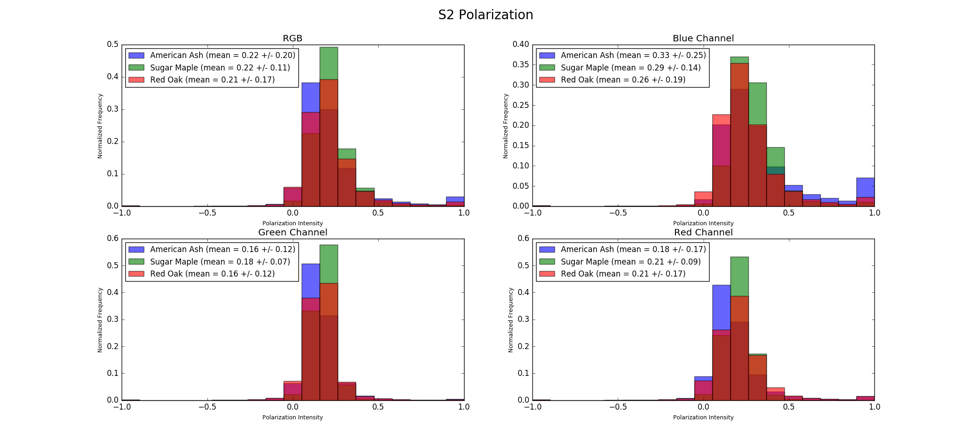
\includegraphics[scale=0.9]{/Sources/Results/7_2_4/S2_polar.png}}
    \end{center}
    \caption{Polarization for all species in the diffuse direction of observation for S2.}
    \label{fig:polarization}
\end{figure}
%
A GLCM analysis in the diffuse direction for all species shows visually distinct clustering.  GLCM dissimilarity and correlation for diffuse scattering can be found in Figure 34.
%
\begin{figure}[!htb]
    \begin{center}
        \makebox[\textwidth]{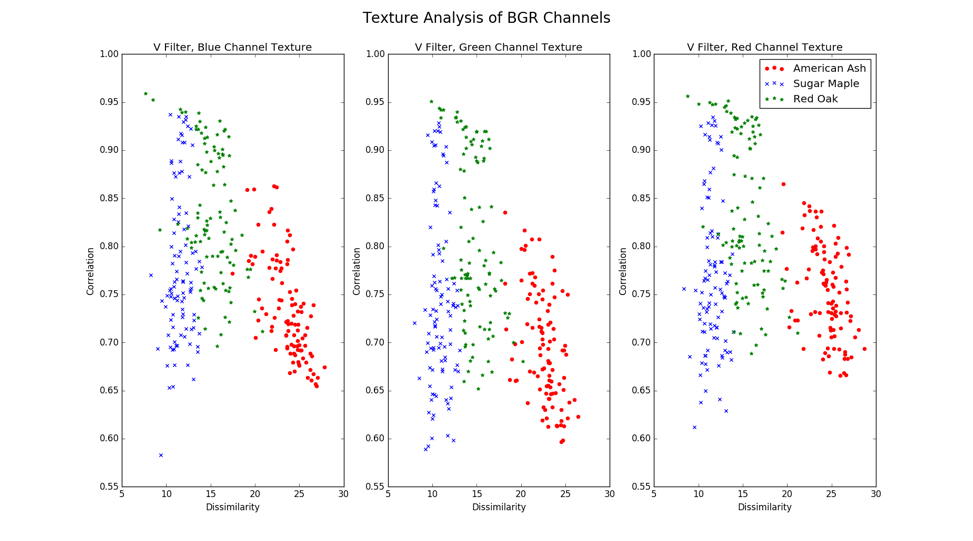
\includegraphics[scale=0.9]{/Sources/Results/7_2_4/glcm.png}}
    \end{center}
    \caption{V filter GLCM dissimilarity and correlation for all species in diffuse direction 0 weeks.}
    \label{fig:polarization}
\end{figure}
%
\subsection{Diffuse Leaf Decomposition}
As the breakdown of the leaf occurs, fewer photons are utilized for photosynthesis.  This results in fewer type B photon interactions as the leaves becomes more reflective.  The diffuse portion of the fresh leaf contains a large amount of type B and C photons.  Intricate structures can be seen in the leaf not seen in the specular images since the diffuse light does not oversaturate the sensor.
%
\begin{figure}[htp]
    \centering
    \hspace*{\fill}%
    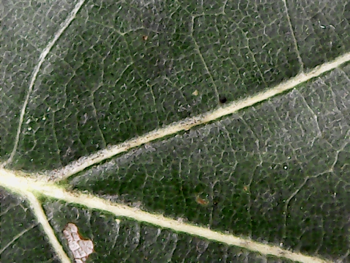
\includegraphics[width=.3\textwidth]{/Sources/Results/7_2_5/oak-0.png}\hfill%
    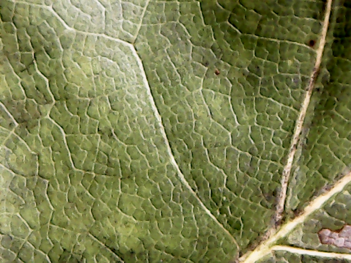
\includegraphics[width=.3\textwidth]{/Sources/Results/7_2_5/red-oak-1.png}
    \hspace*{\fill}%
    \caption{From left to right: Red Oak Freshly Removed and After One Week}
    \label{fig:specular-raw-decompose}
\end{figure}
%
The images above show that in the diffuse direction for Red Oak freshly removed, there are numerous micro segmentations on the leaf surface that were not evident in the specular direction.  These complex wax structures increase the amount of multiple scattering.  As the leaf decomposes, the micro segmentations become less evident as the larger structures become the most prevalent feature on the surface.

Figure 37 and Figure 38 show's the S1 and S2 polarization in the diffuse direction for a Red Oak leaf as it undergoes the decomposition.
%
\begin{figure}[!htb]
    \begin{center}
        \makebox[\textwidth]{\includegraphics[scale=0.9]{/Sources/Results/7_2_5/s1-polar.png}}
    \end{center}
    \caption{Red Oak in the diffuse direction for S1}
    \label{fig:polarization}
\end{figure}
%
The S1 polarization component is low for both the fresh and decomposing leaf in the diffuse direction.  Most of the polarization that results is not purely perpendicular or parallel to the incident surface.  The S and P component of polarization are mostly cancelled out.
%
\begin{figure}[!htb]
    \begin{center}
        \makebox[\textwidth]{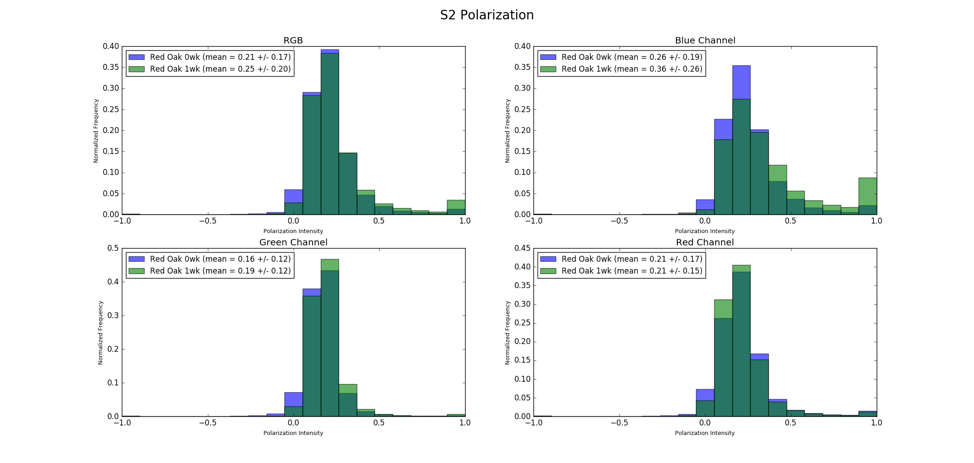
\includegraphics[scale=0.9]{/Sources/Results/7_2_5/s2-polar.png}}
    \end{center}
    \caption{Red Oak in the diffuse direction for S2}
    \label{fig:polarization}
\end{figure}
%
There is S2 polarization that arises from each specimen, and it is shown to be higher for red oak leaves that are undergoing the process of decomposition.

As the composition of a leaf changes, more polarization results as an effect of the physiological breakdown causes less absorption and more volume scattering.  Although diffuse surfaces are supposed to create equal amounts of randomized polarized states, resulting in no overall polarization, it is shown here that in some cases the diffuse portion is polarized, especially in the S2 component.  This information could potentially be useful for determining physiological properties of leaves.

The GLCM in the diffuse direction shows that as the wax structure becomes less filled with water and decompresses, the surface of the leaf appears smoother, since there is less noise caused by multiple scattering through the thicker wax cuticle of the fresh leaves.  The result is that healthier leaves create more dissimilarity for the captured images.  This is shown in Figure 39.
%
\begin{figure}[!htb]
    \begin{center}
        \makebox[\textwidth]{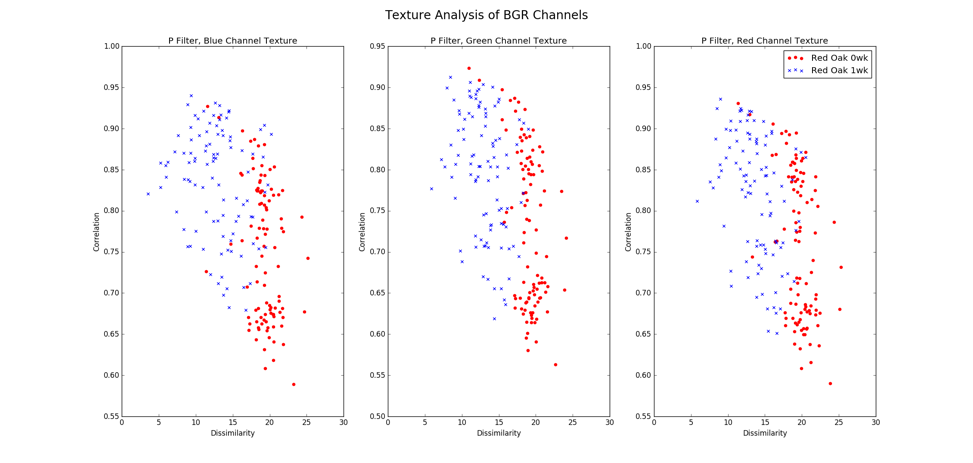
\includegraphics[scale=0.9]{/Sources/Results/7_2_5/glcm.png}}
    \end{center}
    \caption{P filter GLCM dissimilarity and contrast in diffuse direction for red oak 0 week vs 1 week}
    \label{fig:polarization}
\end{figure}
%
The multiple scattering and microstructures evident in the thicker wax of a freshly removed oak leaf creates a high amount of dissimilarity and lower correlation than after a week of drying.

\subsection{Diffuse Classification Results}
Support vector classification was performed on all leaves collected for each of the species with zero and one week combined in order to show the ability to classify similar species even if interclass variance exists.  Overall the diffuse results were slightly less accurate than the specular results, but this may be due to the overall noise in the diffuse images acquired.  Further investigation is required in this regard.

The confusion matrix shows that ash is the most correctly identified class, with the highest precision and recall when compared to other classes.  Classification precision for oak and maple were similar.

The learning curve shows good results as more samples are added, but towards the end shows the score decreases slightly.  Additional samples should be investigated to ensure the validity of this model.

Overall the model proves to be accurate and give the desired results [TODO explain].
%
\begin{figure}[!htb]
    \begin{center}
        \makebox[\textwidth]{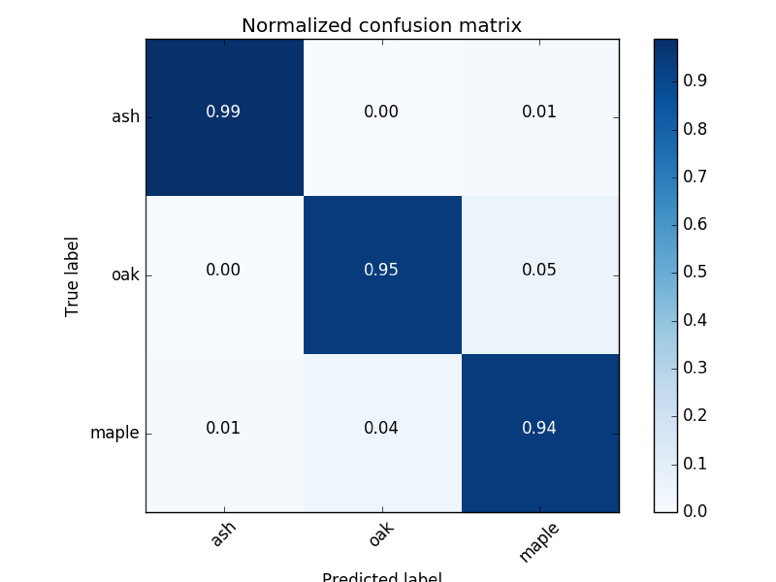
\includegraphics[scale=0.9]{/Sources/Results/7_2_6/confusion.png}}
    \end{center}
    \caption{Confusion matrix for all species observed in the diffuse direction.}
    \label{fig:polarization}
\end{figure}
%
%
\begin{figure}[!htb]
    \begin{center}
        \makebox[\textwidth]{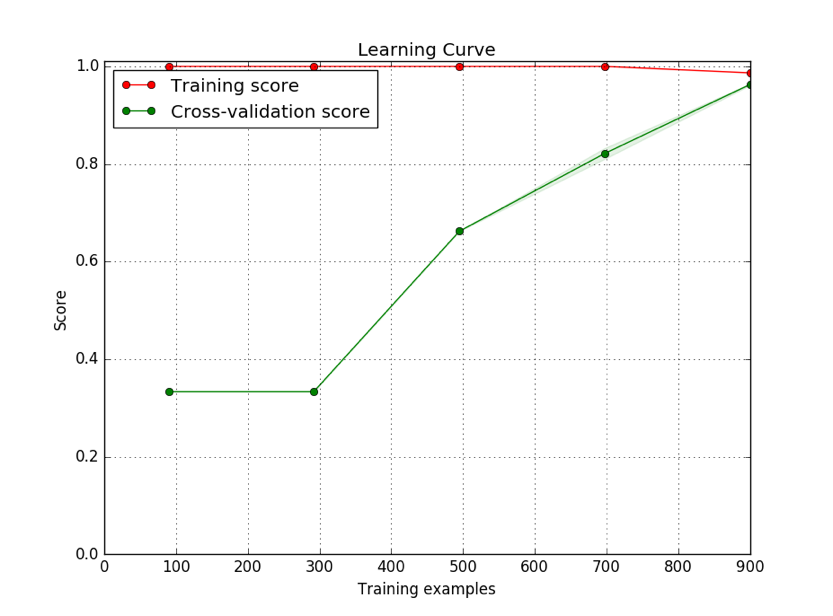
\includegraphics[scale=0.9]{/Sources/Results/7_2_6/learning_curve.png}}
    \end{center}
    \caption{Learning curve for All species observed in the diffuse direction}
    \label{fig:polarization}
\end{figure}
%
%
\begin{table}[htb]
  \centering
  \begin{tabular}{lllll}
    \toprule
    \textbf{Class} & \textbf{Precision} & \textbf{Recall} & \textbf{F1 Score} & \textbf{Support} \\
    \midrule
      \texttt{0.0} & 0.98 & 0.99 & 0.99 & 600 \\
      \texttt{1.0} & 0.93 & 0.94 & 0.94 & 600 \\
      \texttt{2.0} & 0.93 & 0.92 & 0.93 & 600 \\
      \texttt{avg/total} & 0.95 & 0.95 & 0.95 & 1800 \\
    \bottomrule
  \end{tabular}
  \caption{%
    Scores for Classification in the Diffuse Direction with Polarization and Texture in Diffuse Direction.
  }
  \label{tab:Packages}
\end{table}
\begin{table}[htb]
  \centering
  \begin{tabular}{lllll}
    \toprule
    \textbf{Class} & \textbf{Precision} & \textbf{Recall} & \textbf{F1 Score} & Support\\
    \midrule
      \texttt{0.0} & 0.94 & 0.95 & 0.94 & 600 \\
      \texttt{1.0} & 0.90 & 0.92 & 0.91 & 600 \\
      \texttt{2.0} & 0.89 & 0.86 & 0.88 & 600 \\
      \texttt{avg/total} & 0.91 & 0.91 & 0.91 & 1800 \\
    \bottomrule
  \end{tabular}
  \caption{%
    Scores for Classification in the Diffuse Direction with Just Polarization in Diffuse Direction.
  }
  \label{tab:Packages}
\end{table}
%
\begin{table}[htb]
  \centering
  \begin{tabular}{lllll}
    \toprule
    \textbf{Class} & \textbf{Precision} & \textbf{Recall} & \textbf{F1 Score} & Support\\
    \midrule
      \texttt{0.0} & 0.98 & 0.99 & 0.99 & 600 \\
      \texttt{1.0} & 0.77 & 0.85 & 0.81 & 600 \\
      \texttt{2.0} & 0.84 & 0.74 & 0.79 & 600 \\
      \texttt{avg/total} & 0.86 & 0.86 & 0.86 & 1800 \\
    \bottomrule
  \end{tabular}
  \caption{%
    Scores for Classification in the Diffuse Direction with Just Texture in Diffuse Direction.
  }
  \label{tab:Packages}
\end{table}
%
Comparison of with the use of in Table limited feature sets, shows again that texture combined with polarization returns better results than if only one were used.  Overall classification in the diffuse direction was slightly less accurate than that of our specular measurements.

In the future principal component analysis should be utilized to isolate the top parameters for each group in order to eliminate any bias that is caused from there being more polarization features than texture features. An additional image should be acquired with no polarization filter in place, to represent S0 and create a better mark for texture feature only comparison.

\section{Regression}
Previous results show that classification between species can be performed with high levels of accuracy even if a large amount of interclass variance exists due to varying physiological states of each leaf.  Therefore, investigation into acquiring more accurate measures as to the plants' current physiological state, such as water and pigment concentration, would be useful for a more detailed explanation of previous results.

Determining the relationship between the relative water content of a plant's leaf, versus features extracted from images taken in the visible portion of the spectrum with a camera, requires data to be fit in a regression model.  Support Vector Regression (SVR) is an extension of linear regression with the purpose of minimizing the distance of each point to the best fit line.

The y dependent variable was determined by measuring the relative water content of the Devils Ivy plant using the procedure previously described.  Samples were extracted from each polarization filter for the purpose of GLCM analysis.  The average dissimilarity, contrast, energy and correlation of 100 samples randomly selected from the entire image were utilized to quantify the texture of each individual leaf at different levels of RWC.  The S1 and S2 polarizance parameters were also calculated for each individual pixel. Each pixel was binned together to create histograms for S1 and S2.  The probabilities for 20 bins ranging from -1 to 1 were utilized to determine the polarization component of each sample.

Principal component analysis was utilized to extract the most useful features for plotting against the RWC.  The principal component can be seen plotted against RWC for the specular case in Figure 42.
%
\begin{figure}[!htb]
    \begin{center}
        \makebox[\textwidth]{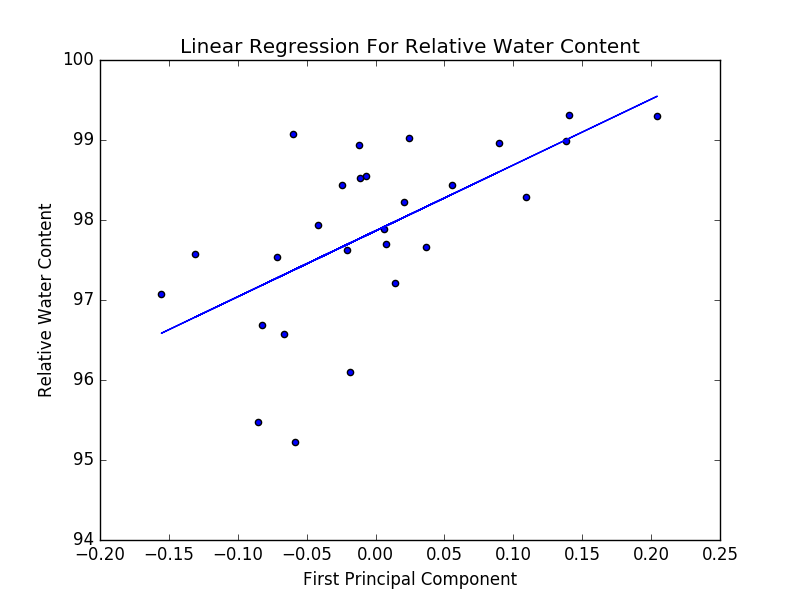
\includegraphics[scale=0.9]{/Sources/Results/rwc-regression.png}}
    \end{center}
    \caption{Linear Regression for RWC and 1st principal component}
    \label{fig:polarization}
\end{figure}
%
%
\begin{table}[htb]
  \centering
  \begin{tabular}{ll}
    \toprule
    \textbf{Metric} & \textbf{Score}\\
    \midrule
      \texttt{r2} & 0.376 \\
      \texttt{RMS} & 0.758 \\
    \bottomrule
  \end{tabular}
  \caption{%
    Scores for Regression in the Specular Direction
  }
  \label{tab:Packages}
\end{table}
%
Analyzing the specular polarization and extracting texture features showed good results [TODO why? what exactly are results].  The classifier was cross validated using K fold validation with 10 folds.  The performance of the classifier is summarized in Table.
%todo add table and explain each attribute
The root mean squared shows the accuracy [TODO explain accuracy] to be within 0.5% of the actual value for the predicted linear model.  The classifier was initialized with the parameters
%TODO add code
These parameters were acquired by performed a grid search that optimizes for the root mean square error.

Further data is required to more accurately fit this model, although the initial results are promising.

  %%%%%%%%%%%%%%%%%%%%%%%%%%%%%%%%%%%%%%%%%%%%
\chapter{Conclusion}
%%%%%%%%%%%%%%%%%%%%%%%%%%%%%%%%%%%%%%%%%%%%
\begin{center}
  \begin{minipage}{0.75\textwidth}
    \begin{small}
      “It would not be much of a universe if it wasn't home to the people you love.”\\
      \null\hfill\emph{Stephen Hawking}
    \end{small}
  \end{minipage}
  \vspace{0.5cm}
\end{center}

The need for precisely monitoring the health of vegetation will grow as resources become more scarce.  Precision agricultural will become a necessity for human survival. The sensing technologies involved with satellites, drones, and indoor greenhouses provide information that contribute to our understanding of photon vegetation interactions. Information captured by these sensors occur at numerous scales. Understanding the micro and macro level effects involved with these interactions allow for the potential to gain deeper understanding into the natural world around us. The data acquired is useful for determining the physiological status of plants in different environments under low resource conditions. Lower resources will require a decrease in the wasting of inputs involved with producing food and other agricultural outputs.

A large amount of research previously conducted has focused on large scale imaging techniques for analyzing data acquired from satellites and drones.  Texture has been used in remote sensing technologies for the purpose of classifying the various terrains and structures within an image.  The inclination to bring these ideas to microscale agricultural systems in greenhouses throughout the solar system can be useful going forward as interest in this field grows.  The complexity of the microscale interactions today is largely ignored.  As models have a need to grow in realization and complexity their will be a need to explain the nuances of the macro level data.  Small scale data acquisition and analysis is critical for understanding these effects.

As areas in precision agriculture expand into areas of indoor growing operations in more controlled environments, the application of precise amounts of agricultural inputs will become more viable.  A better understanding of the effects of light on individual plants for determining their overall health will be useful in the future as resources become more scarce.

This research has set a foundation for discussion surrounding the information to be gained from observing the polarization response, at a micro level, that results from incident unpolarized light onto a leafs surface.  This type of interaction is found naturally but for controlled, experimental purposes is created in a lab setting. Images were acquired with plants in various physiological conditions including decomposition and water stress.  As these conditions change, the physiology of each leaf on the plant also change.  Cellular structures begin to break down and influence the polarization of the reflected radiation.  The texture of the leafs surface was also observed to change as these processes progressed.

The polarization created by a material when unpolarized light is incident, as in most natural settings, has been shown to reveal distinguishing characteristics for determining both the species and physiological state of vegetation.  Although normally assumed to be unpolarized, the diffuse portion of reflectance contains information that can be useful for classification and plant health analysis.  The specular portion of light also contains distinguishing information and in our results provided better classification.

The initial assumption of the diffuse portion of light being an unpolarized, scattering mechanism has been recognized in recent years as being a simplification of the scattering mechanisms.  It is akin to assuming the specular portion is completely polarized; an idealization and not an observation.  New experimentation and research into the diffuse reflectance of a wide variety of materials and substances shows that information collected contains insight into the properties of these materials. These properties are shown to be useful for classification and staging purposes.

The relative water content of leaves is shown to be correlated with both its texture and polarization response when captured by a digital microscope behind a rotating linear polarizer. Results for Red Oak have been provided in detail for this report as it provides the simplest explanation for the results.  Each species provides slightly different results depending on its composition.  Further explanation would have to be given at an individual species level to account for these results.

Further improvements to experiment design, plant health status control, image acquisition and segmentation should be taken to improve the results of regression.  Plants can be controlled at a finer level when grown by starting seeds in a controlled environment.  Inputs to each individual plant could be altered including various fertilizers and water amounts.  Paper chromatography methodologies, as discussed in \cite{pigments}, could be used for determining the various distribution of pigments throughout smaller subsections of the leaves.  By creating false images with polarization and texture information, smaller sections of leaves could be isolated and correlated with each feature.  Image acquisition could be improved by reducing the amount of undulations on a leafs' surface in order to reduce the number of effects that arise from masking and shadowing.  Different light sources should be investigated to determine the consistency of our results.  Image segmentation may prove beneficial in isolating the effects of localized features.  Physiological indicators such as pigment concentrations in addition to relative water content should be investigated to further show health status and correlate the polarization response.

In the area of polarization and texture modeling, examples could be given as to how various textures, such as sandpaper, glass, etc. are related to their polarization response in a simplistic model.

Overall this study has provided a basis for many of the principles required for understanding the microscale concepts involved with the sensing of vegetation. Improvements to current models and suggestions for areas of further study have been provided.
\\
It is not the man that lives on, but the mold.


% This ensures that the subsequent sections are being included as root
% items in the bookmark structure of your PDF reader.
\bookmarksetup{startatroot}
\backmatter

  \begingroup
    \let\clearpage\relax
    \glsaddall
    \printglossary[type=\acronymtype]
    \newpage
    \printglossary
  \endgroup

  \printindex
  \printbibliography

\end{document}
